%-------------------------------------------------------------------%
%                      filename: skeleton.tex                       %
%-------------------------------------------------------------------%
\documentclass[aps,twocolumn]{revtex4-1}
\usepackage{graphicx}
\usepackage{ifpdf}
\ifpdf
	\usepackage[backref]{hyperref}
	%\usepackage[backref,pageanchor=true,plainpages=false, pdfpagelabels,bookmarks,bookmarksnumbered]	{hyperref}
\else
\fi

\usepackage{crs}

% see http://goo.gl/5Fo27
\newtoggle{thmsty}
%\toggletrue{thmsty}
\togglefalse{thmsty}

% see http://goo.gl/7jLZ9
\makeatletter
\newlength \figwidth
\if@twocolumn
  \setlength \figwidth {0.8\columnwidth}
\else
  \setlength \figwidth {0.5\textwidth}
\fi
\makeatother

\begin{document} 

\title{\bf Coherence constraints on hierarchical transitions in evolutionary processes}

\author{a1$^{1}$, a2$^{1}$, a3$^{1}$, a4$^{1,2,3}$}

\affiliation{$^1$Department of Systems and Computational Biology,\\ $^2$Dominick P. Purpura Department of Neuroscience, \\ $^3$Department of Pathology, Albert Einstein College of Medicine, 1301 Morris Park Ave, Bronx, NY 10461, USA}

\date{\today}
\begin{abstract}
Hierarchy is a fundamental organizing concept in biology. The existence of a number of apparently {\it discrete} levels of organization including molecules, cells, organisms, populations, communities, ecosystems, and more fine-grained levels below, above and in between these are taken for granted. Theoretical constructs capable of integrating information about such levels of organization and of explaining the emergence of such levels in the evolutionary process have not been adapted to a biological context. Here we make use of existing theory to characterize coherence constraints that must ostensibly be satisfied in any evolutionary process in which two levels of organization become coupled such that one serves as a base supporting the existence of and providing potential for interactions among higher-level entities in another. In this way, what may be considered as two distinct levels may come to be viewed as part of a unified system. This process of unification of distinct levels may serve as a basis for induction in the consideration of arbitrarily complex compositions of multilevel biological systems. The language we use to express these constraints is sufficiently general that it applies equally to several different concrete formalisms for representing biological systems, for example those that have become commonplace in the context of network science, in terms of algebraic graphs, hypergraphs, or (cell) complexes. This constraint on the relationship between levels of organization in static representations of {\it biological networks} may be able to be used to provide boundary conditions for dynamical models---for example those defined in terms of transformations on graphs---that seek to take into account transitions in hierarchical organization that occur in some types of evolutionary processes.
\end{abstract}

\maketitle

\tableofcontents

\section{Reasoning about emergent properties of biological systems}

The development of a formal language for modeling and reasoning about biological systems was suggested by Joseph Woodger in collaboration with the developmental biologist Conrad Waddington and the logician Alfred Tarski as early as 1937~\cite{Woodger1937,Woodger1951,Woodger1952,Woodger1952a}. At that time it was perhaps difficult to understand how such a language could be put to use. Today we have tools that could enable the use of such a language: namely 1) computational machines to automate the details of routine transformations within the language and 2) accessible, growing repositories of biological data. Though we have access to necessary infrastructure, we lack such a language suggested by Woodger and others throughout the course of the 20th century as we have continued to rely on natural language heuristics to communicate and reason about biological systems.

Category theory~\cite{Lane1985,Lane1998,MacLane1992,Lawvere1997,Lawvere2003,Awodey2006} is a language that has been suggested since Woodger to provide a framework for representing and reasoning about biological systems~\cite{Rashevsky1954,Rosen1958,Rosen1958a,Rosen1978,GOGUEN1979,Rosen1985,Rosen1991,Ehresmann2007,Louie2009}. What is immediately useful about this language from the perspective of biology and its underlying chemistry is that it presents as primitive the notion of transformation between objects. In fact, from this point of view, a defining characteristic of any representation of an entity (e.g. a protein, cell, organism, or population) is the set of relationships between its representations of other entities under consideration. Intrinsic properties are taken into account implicitly in this framework since the possible set of relationships between any object and any other is constrained by the nature of its intrinsic properties. 

Concepts from category theory, especially with regard to its interface with geometry and logic~\cite{MacLane1992,Jacobs1998}, enable the formulation of what might be viewed as a framework for explaining the nature and development of so-called \emph{emergent properties} of systems that are able to represent information in molecular terms~\cite{Harmer2010}, to consider an arbitrary {\it base} level, but build upon this to generate the capacity to process information at higher levels of organization, such as the cellular or multicellular, as well. The existence of biological {\it levels of organization} that may have come into existence during the evolutionary process thus far, although commonly assumed for example in various formal and informal taxonomic systems used in biology, is a hypothesis that should be able to be tested in the long term through the introduction of a language capable of making predictions that could help distinguish a case in which there is from that in which there is no justification to reify the conceptual levels of organization that have been introduced to organize biological knowledge.

The concept of separation of spatio-temporal scales, which is used to justify approximate isolation of particular levels of organization in the process of constructing models of restricted biological subsystems~\cite{Gunawardena2012,Karr2012} may make it impossible to explain evolutionary processes that apparently transcend such levels of organization providing one justification to search for a language able to support model-building that can offer explanations for how biological systems might integrate information across levels of organization, as it obviously appears they must in order to satisfy necessary conditions for their existence. The methods discussed here are general enough that they can be equally well applied to the consideration of relationships, assuming there are any at all, among any levels of biological organization. Of course, this framework will require specialization to be of use in particular contexts. It may ultimately become more useful for building concrete models that can be directly compared to experimental data, to formulate ideas analogous to those discussed here in terms of non-equilibrium statistical mechanics~\cite{Ellis1985,Freidlin1998,Touchette2009,Smith2011}. However, the unity deriving from the judicious definition of concepts underlying category theory {\it per se} is precisely the type of abstraction we argue is necessary to enable a compression of concepts, and, thereby, improve our capacity to organize, communicate, and synthesize existing and future knowledge about extant biological systems. Furthermore, such abstractions may support the extraction of invariants of evolutionary processes, even if such invariants may require expression in terms of higher-order logics, potentially enabling the evaluation of this information with respect to the spectrum bounded by evolutionary necessity and historical contingency~\cite{Fontana1994,Fontana1994a,Fontana1996}.

Here we explain concepts from category theory necessary to understand the way in which mathematical representations of interacting objects at one level of organization (e.g. molecules) can produce phenomena that would themselves be identifiable as derived objects (e.g. cells) that justify the very conceptualization of a \emph{level of organization} in the first instance. We focus exclusively on defining the boundary conditions relating levels of organization (e.g. molecules to cells or cells to multicellular organisms), which are necessary to understand in the course of defining a dynamical system rooted in transformations operating on structured objects rather than relatively less-structured quantities that could model the \emph{evolution} of such \cite{Fontana1994,Fontana1994a,Fontana1996}. What results is a refinement of the way in which levels of organization may be conceptually discriminated and related. This capacity is important since such concepts are ubiquitously employed in biology, even if they are, so far, used only heuristically as guides to pre-existing intuition (e.g. in the hierarchical nature of taxonomy or in the characterization of transcriptional and epigenetic among other potential levels of regulation of gene expression). Understanding how information is integrated via biological processes across such levels of organization is fundamental to the understanding of so-called complex phenotypes and the associated set of contingencies necessary to account for in any proposed methods targeted at controlling or otherwise manipulating them.

\section{Information representation and transformation in biological systems}

\begin{quotation}
{\it One [...] idea, which underlies everything in this book, is the concept
of genomically encoded information processing. [...],
this is like the geological basis of the landscape. In my view, cis-regulatory information processing, and information processing at the gene regulatory network circuit level, are the real secret of animal development. Probably the appearance of genomic regulatory systems capable of information processing is what made animal evolution possible.} -Eric H. Davidson~\cite{Davidson2006a}
\end{quotation}

%\subsection{System-environment duality}
Distinction between biological systems or some components thereof and the environments within which they are embedded is implied in models of such systems. This distinction is useful in many contexts, but the boundary between a biological system and its environment is dependent upon the level of resolution taken by any particular \emph{model} and \emph{modeler} independent of its relationship to properties of biological systems themselves~\cite{Fontana1996}. In this light, it is desirable to develop a modeling framework for biological systems that supports variation of this boundary without requiring the development of structurally independent models. Constructing a framework for such models requires the determination, unification, and incorporation of abstract features of biological systems that are invariant across levels of organization from molecules to cells, organisms, populations, communities, ecosystems and more fine-grained levels of resolution that likely lie between these broadly and imprecisely defined perspectives one can take with regard to representing biological systems. This capacity already exists within and is the primary potential utility of so-called network representations of biological systems; however, what needs to be imported into this context is the use of algebraic methods to enable reasoning and subsequent hypothesis development about such network representations for the purpose of coupling such modeling methods into feedback loops with empirical ones.

\begin{figure*}
\noindent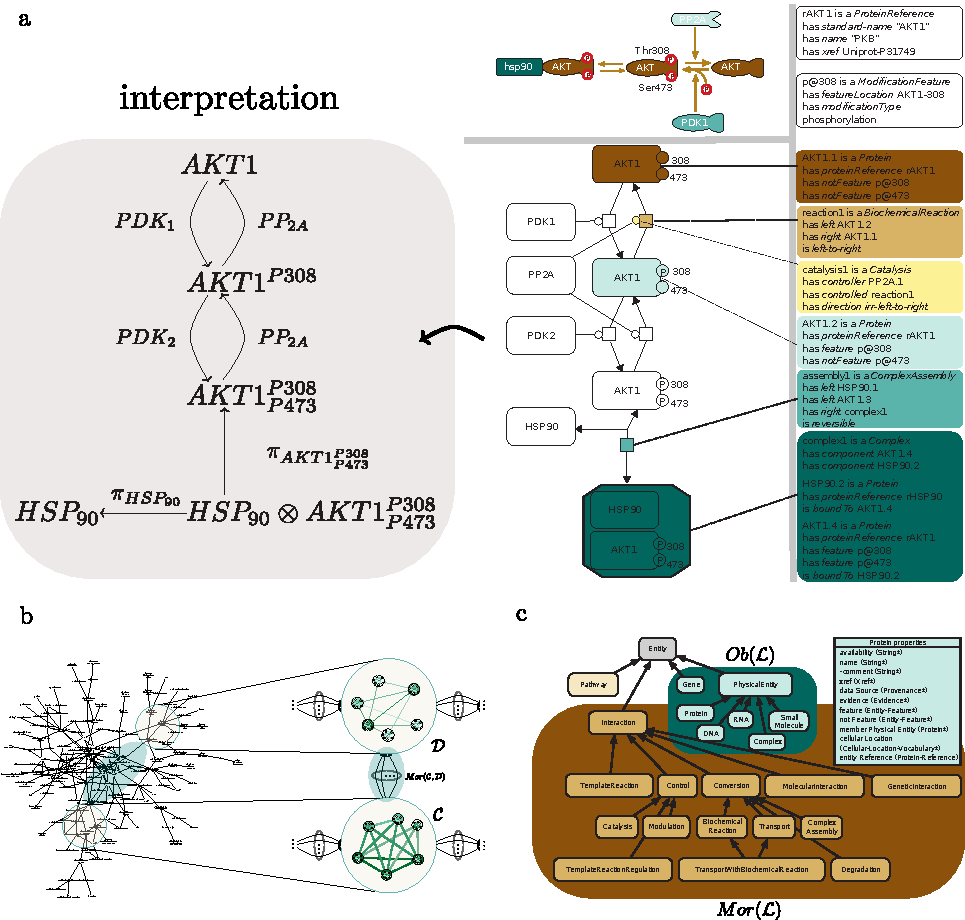
\includegraphics[width=2\columnwidth]{fig/Fig1Composite.pdf}
\caption{Particular motifs within interaction networks underlying biological systems can be abstracted as algebraic structures of some type exhibiting internal structure associated to that type and external structure, which may reflect aspects of the internal structure, represented by morphisms translating structure between them. (a) We provide an example of a simple categorical semantics (left) for the BioPAX ontology~\cite{Demir2010} (right) of some of the interactions involved in the Akt pathway. (b) A representation (left) of the integrated metabolic-gene regulatory glycolytic network of E. coli K12 MG1655 derived from the EcoCyc database~\cite{Keseler2011} in terms of the BioPAX ontology a conceptual picture (right) of the way in which the relationships between substructural motifs of a particular network can be represented algebraically in terms of algebraic structures that can be referred to as objects and methods of transforming or mapping between these structures referred to as morphisms. (c) The broadest distinctions in the BioPAX ontology between {\it physical entities} and {\it interactions} corresponds to the typing distinction in category theory between {\it objects} and {\it morphisms}. Panels (a, right) and (c) are reproduced from~\cite{Demir2010}.}
\label{fig:biograph}
\end{figure*}

%\subsection{Transformation of information via adjoint functors}
The use of category theoretic adjunctions to model intrinsic information representation in biological systems has been suggested~\cite{GOGUEN1979,Ellerman2005}, but these efforts have yet to be incorporated into theories that attempt to make contact with {\it status quo} ontology for biological data~\cite{Demir2010} and also allow for potential {\it hierarchical} information representation. This is likely in part a result of the difficulty in specifying the appropriate level of abstraction at which a precise metaphor can be developed between collections of interacting biological entities and a particular type of mathematical structure. A very promising approach has been developed in the context of so-called general systems~\cite{Zafiris2005a,Zafiris2005b,Zafiris2012}. The metaphor described in that context needs to be clarified in order to adapt it to a biological context, which may include specializing to, but will ideally involve integrating information about, molecular, signaling, gene regulatory, and other interaction networks that underly biological systems toward the goal of making the theory comparable to experimental data. We begin here by developing the prerequisite definitions to explain why the transformation of biological information across an arbitrarily specified system boundary is naturally represented as a pair of adjoint functors in the context of category theory. A relevant piece of intuition to associate to what follows is that any interaction between biological entities potentially establishes prerequisite value to high- or low-fidelity transmission and representation of information regarding the state of other collections of spatio-temporally distant interactions. The participants in such an interaction may ultimately require representation as categories themselves because underlying each may be arbitrarily related collections of interactions that are necessary for the existence of the interface implicit to specifying such an interaction. This situation may eventually require the introduction of higher categories~\cite{Lein2004}, but here we maintain a simpler assumption that such interacting entities can be modelled as objects in a category and leave this potentially useful or necessary generalization to future work.

Many details of the technical background are presented in Appendix \ref{app:CatTh}. Here we present a minimal collection of definitions necessary for the proceeding discussion.
\iftoggle{thmsty}{
\begin{definition}
\label{definition-category}
}{}
A {\it category} $\mathcal{C}$ is:
\begin{enumerate}
\item A set of objects $\Ob(\mathcal{C})$.
\item For each pair $x, y \in \Ob(\mathcal{C})$ a set of morphisms
$\Mor_\mathcal{C}(x, y)$.
\item For each triple $x, y, z\in \Ob(\mathcal{C})$ a morphism represeting composition
$ \Mor_\mathcal{C}(y, z) \times \Mor_\mathcal{C}(x, y)
\to \Mor_\mathcal{C}(x, z) $, denoted $(\phi, \psi) \mapsto
\phi \circ \psi$.
\end{enumerate}
Such that the following are satisfied:
\begin{enumerate}
\item For every element $x\in \Ob(\mathcal{C})$ there exists a
morphism $\text{id}_x\in \Mor_\mathcal{C}(x, x)$ such that
$\text{id}_x \circ \phi = \phi$ and $\psi \circ \text{id}_x = \psi $.
\item Composition is associative, i.e., $(\phi \circ \psi) \circ \chi =
\phi \circ ( \psi \circ \chi)$.
\end{enumerate}
\iftoggle{thmsty}{
\end{definition}
}

\iftoggle{thmsty}{
\begin{definition}
\label{definition-functor}
}{}
A {\it functor} $F : \mathcal{A} \to \mathcal{B}$
between two categories $\mathcal{A}, \mathcal{B}$ is:
\begin{enumerate}
\item A morphism $F : \Ob(\mathcal{A}) \to \Ob(\mathcal{B})$.
\item For every $x, y \in \Ob(\mathcal{A})$ a map
$F : \Mor_\mathcal{A}(x, y) \to \Mor_\mathcal{B}(F(x), F(y))$,
denoted $\phi \mapsto F(\phi)$.
\end{enumerate}
These data should be compatible with composition and identity morphisms: $F(\phi \circ \psi) =
F(\phi) \circ F(\psi)$ for a composable pair $(\phi, \psi)$ of
morphisms of $\mathcal{A}$ and $F(\text{id}_x) = \text{id}_{F(x)}$.
\iftoggle{thmsty}{
\end{definition}
}

\iftoggle{thmsty}{
\begin{definition}
\label{definition-transformation-functors}
}{}
Let $F, G : \mathcal{A} \to \mathcal{B}$ be functors.
A {\it natural transformation}, or a {\it morphism of functors}
$t : F \to G$, is a collection $\{t_x\}_{x\in \Ob(\mathcal{A})}$
such that
\begin{enumerate}
\item $t_x : F(x) \to G(x)$ is a morphism in the category $\mathcal{B}$, and
\item for every morphism $\phi : x \to y$ of $\mathcal{A}$ the following
diagram is commutative
$$
\xymatrix{
F(x) \ar[r]^{t_x} \ar[d]_{F(\phi)} & G(x) \ar[d]^{G(\phi)} \\
F(y) \ar[r]^{t_y} & G(y) }
$$
\end{enumerate}
\iftoggle{thmsty}{
\end{definition}
}

We can define a category having functors as objects and natural transformations as morphisms, which is called a functor category, by recognizing that every functor $F$ comes with the {\it identity} transformation $\text{id}_F : F \to F$. In addition, given a morphism of
functors $t : F \to G$ and a morphism of functors $s : E \to F$
then the {\it composition} $t \circ s$ is defined by the rule
$$
(t \circ s)_x = t_x \circ s_x : E(x) \to G(x)
$$
for $x \in \Ob(\mathcal{A})$.
This is a morphism of functors
from $E$ to $G$.
Thus, given categories
$\mathcal{A}$ and $\mathcal{B}$ we obtain the category of functors between $\mathcal{A}$ and
$\mathcal{B}$.

\iftoggle{thmsty}{
\begin{definition}
\label{definition-equivalence-categories}
}{}
An {\it equivalence of categories}
$F : \mathcal{A} \to \mathcal{B}$ is a functor such that there
exists a functor $G : \mathcal{B} \to \mathcal{A}$ such that
the compositions $F \circ G$ and $G \circ F$ are isomorphic to the
identity functors $\text{id}_\mathcal{B}$,
respectively $\text{id}_\mathcal{A}$.
In this case we say that $G$ is a {\it quasi-inverse} to $F$.
\iftoggle{thmsty}{
\end{definition}
}

\iftoggle{thmsty}{
\begin{definition}
\label{definition-adjoint}
}{}
Let $\mathcal{C}$, $\mathcal{D}$ be categories.
Let $F : \mathcal{C} \to \mathcal{D}$ and
$G : \mathcal{D} \to \mathcal{C}$ be functors.
We say that $F$ is a {\it left adjoint} of $G$ or that
$G$ is a {\it right adjoint} to $F$, written $F \dashv G$, if there are bijections
$$
\phi_{c,d}:\Mor_\mathcal{D}(Fc, d)
\simeq
\Mor_\mathcal{C}(c, Gd)
$$
functorial in $c \in \Ob(\mathcal{C})$, and
$d \in \Ob(\mathcal{D})$.
\iftoggle{thmsty}{
\end{definition}
}

Morphisms that are associated with each other according to the bijections of an adjunction are called {\it adjoint transposes} of one another. If $g:Fc \rightarrow d$, $g \in \Mor(\cD)$ then $g^*: c \rightarrow Gd$, $g^* \in \Mor(\cC)$ is given by $\phi_{c,d}(g) = g^*$. Similarly for $f: c \rightarrow Gd$, $f \in \Mor(\cC)$ with $f^*:Fc \rightarrow d$, $f^* \in \Mor(\cD)$ is given by $\phi_{c,d}^{-1}(f) = f^*$. We see then that $g^* = f$ and $f^* = g$.

\iftoggle{thmsty}{
\begin{definition}
\label{definition-unit}
}{}
Consider the identity morphism $1_{Fc} \in \Mor_{\cD}(Fc,Fc)$. The adjoint transpose of $1_{Fc}$ is the {\it unit} morphism at $c$
$$
\phi_{c,Fc}(1_{Fc})=1_{Fc}^*=\eta_c: c \rightarrow GFc
$$
where $\eta_c \in \Mor_{\cC^{opp}}(c,GFc)$, which, when taken to be natural in $c \in \Ob(\cC^{opp})$, gives the natural transformation
$$
\eta : 1_{\cC^{opp}} \Rightarrow GF
$$
\iftoggle{thmsty}{
\end{definition}
}

\iftoggle{thmsty}{
\begin{definition}
\label{definition-counit}
}{}
Consider the identity morphism $1_{Gd} \in \Mor_{\cC^{opp}}(Gd,Gd)$. The adjoint transpose of $1_{Gd}$ is the {\it counit} morphism at $d$
$$
\phi_{Gd,d}^{-1}(1_{Gd})=1_{Gd}^*=\epsilon_d: FGd \rightarrow d
$$
where $\epsilon_d \in \Mor_{\cD}(d,FGd)$, which, when natural in $d$, gives the natural transformation
$$
\epsilon: FG \Rightarrow 1_{\cD}
$$
\iftoggle{thmsty}{
\end{definition}
}

\begin{figure}
\noindent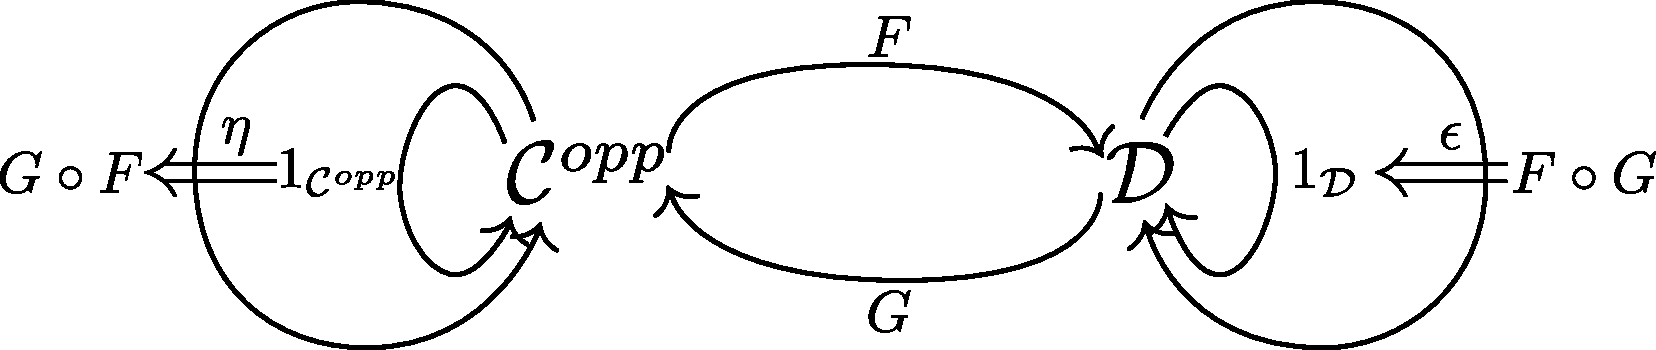
\includegraphics[width=0.9\columnwidth]{fig/adjunction.pdf}
\caption{The adjoint relationship between functors $F \dashv G$ with unit $\eta$ and counit $\epsilon$ natural transformations. The asymmetry in the encoding-decoding relationship indicates that $FG \cD$ can be translated back into the original terms of $\cD$ whereas $GF \cC^{opp}$ cannot necessarily be translated back into the original terms of $\cC^{opp}$.}
\label{fig:adjunction}
\end{figure}

In this framework, information encoding/decoding is an asymmetric process that can only be accomplished without loss of information in one direction: objects of $\cD$ can be encoded into objects of $\cC$ and decoded into objects of $\cD$ but, in general, proceeding in the opposite order may result in loss of information. The asymmetry of the adjunction can be dispensed with if the unit and counit natural transformations are in fact natural isomorphisms $\eta: 1_{\cC^{opp}} \cong GF$ and $\epsilon: FG \cong 1_{\cD}$. In any limit in which this is the case the adjunction $F \dashv G$ gives an equivalence of categories $\cC^{opp} = \cD$ and the information encoding-decoding process becomes bidirectionally exact.

%\section{A topological framework for biological information}

\section{Hierarchical biological information representation}
%% cite something explaining the concept of operationalism as intrinsic
%% to interactions comprising biological systems
Collections of interacting biological entities can be viewed as performing measurements and representing information derived from such measurements on other collections (figure \ref{fig:infopres}). This perspective can be abstractly referred to as intrinsic operationalism, where the components of biological systems take on the role of the measurements they are capable of performing on and representing in terms of one another~\cite{Wolkenhauer2007,Houle2011}. We qualitatively associate an algebraic structure to the relatively primitive biological entities under consideration that provide a {\it local} description with respect to a {\it global} description which may be represented by a composite algebraic structure of observables that can be constructed by potentially gluing together components from those defined locally. This perspective suggests the capacity to both deconstruct and resynthesize composite systems in terms of locally and globally defined algebraic structures.

The approach outlined above can, in principle, be iterated over multiple local-global transitions where in ascending from bottom to top global objects and the associated measurements they are capable of performing in terms of one another become local objects when the perspective is shifted to the next level of organization. It is thus helpful to consider a method for representing the way in which collections of interactions can be woven together to produce higher-order structures that are also capable of interacting with one another. This capacity will be taken advantage of to define a structural condition abstractly characterizing a coherence constraint that must be satisfied by systems that can be considered to be comprised of two or more hierarchically related levels of organization. Such a representation is likely relevant to understanding and constructing models of so-called major transition in evolution~\cite{MaynardSmith1995,Okasha2006,Calcott2011}, but depending upon the way in which hierarchy is to be represented and understood, it may be relevant to much more fine-grained evolutionary changes \cite{Ravasz2002,Guimera2005,Bhardwaj2010}. For now, in order to describe the generic relationship between one collection of local entities and another collection of global entities that are composite constructions upon modules or {\it diagrams} defined on the collection of local entities, we first construct a category for each of the local and global levels of interaction, $\mathcal{L}_0$ and $\mathcal{L}_1$, respectively. It may be intuitive to consider that all the structure in $\mathcal{L}_0$ may be recapitulated in $\mathcal{L}_1$ and not conversely, but this is not explicitly imposed.

\begin{figure}
\noindent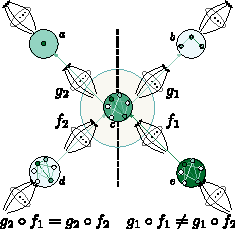
\includegraphics[width=0.9\columnwidth]{fig/infopres.pdf}
\caption{From bottom to top and on the left we imagine an information non-preserving interaction resulting from the inability of $a$ to distinguish in subsequent or {\it downstream} interactions the interaction of $d$  with $c$ from that of $e$ with $c$, whereas on the right we imagine an information preserving interaction wherein $b$ is capable of distinguishing in downstream interactions the interaction of $d$  with $c$ from that of $e$ with $c$.}
\label{fig:infopres}
\end{figure}

%\subsection{Intrinsic perspectives on biological information representation}

The relationship between local and global biological information representations is expressed in terms of a relationship between the categories $\mathcal{L}_0$ and $\mathcal{L}_1$. We can construct a method for relating local and global biological information contained in these two categories. The Yoneda embedding of a category into its associated category of presheaves by the functor $PSh$ and the associated lemma guaranteeing that any category is a full subcategory of its category of presheaves for an arbitrary category is explained in appendix \ref{app:CatTh}, which we specialize to the case of $\mathcal{L}_0$ as $PSh: \mathcal{L}_0 \rightarrow \textit{Sets}^{\mathcal{L}_0^{opp}}$. We abstractly define a functor to be constructed $A:\mathcal{L}_0 \rightarrow \mathcal{L}_1$ that assigns global information representations and morphisms that preserve the structure between them to those of local information representations with respect to a biological system.  Similarly, the functor $R: \mathcal{L}_1 \rightarrow \textit{Sets}^{\mathcal{L}_0^{opp}}$ assigns presheaves on $\mathcal{L}_0$ to the composite information representations in $\mathcal{L}_1$ and $L$ acts in the opposite direction. The categories of local and global information representation and the functors enabling partial translation between them is summarized in figure \ref{fig:ascent}.

In order to construct the functor $L$, we need to explain the relationship between objects in the category of presheaves and the representable functors from their underlying category.

\begin{figure}
\noindent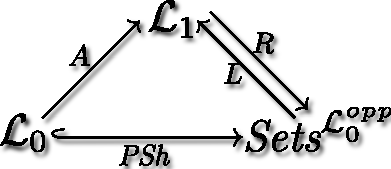
\includegraphics[width=0.5\columnwidth]{fig/ascent.pdf}
\caption{A framework for the construction of a mechanism of local-global translation of biological information. $\mathcal{L}_0$ and $\mathcal{L}_1$ are respectively the categories of relatively local and global biological information representations. The Yoneda embedding functor $PSh$ constructs the presheaf functor category on $\mathcal{L}_0$. The functors $A$, $R$, and $L$ are initially defined abstractly and subsequently constructed.}
\label{fig:ascent}
\end{figure}

\iftoggle{thmsty}{
\begin{definition}
\label{definition-category-of-elements}
}{}
For any category $\mathcal{C}$, {\it index} or {\it diagram} category $J$, and functor $D:J \rightarrow \cC$, every $P \in \Ob(\textit{Sets}^{\cC^{opp}})$ is a colimit of $\cC$-representable functors
$$
\lim\limits_{\overrightarrow{j \in J}} PSh D_j \cong P.
$$
This means there is a unique choice for $J$ and $D$ such that
$$
\lim\limits_{\longrightarrow{J}} PSh \circ D \cong P.
$$
The unique index category $J$ that serves to render the above statements true is called the {\it category of elements} of the presheaf $P$ and is denoted
$$
\int_{\cC} P.
$$
The objects of $\int_{\cC} P$ are pairs $(C,x)$ where $C \in \Ob(\cC)$ and $x \in PC$. The morphisms are triples $(g,(C',x'),(C,x))$ where $g:(C',x') \rightarrow (C,x)$ derives from $g: C' \rightarrow C \in \Mor(\cC)$ and these satisfy the condition
$$
P(g)(x)=x'.
$$
There is also a projection functor that recovers structure in $\cC$ from the category of elements of $P$
$$
\pi : \int_{\cC} P \rightarrow \cC
$$
defined on objects and morphisms of the category of elements of $P$ respectively as $\pi(C,x)=C$ and $\pi (g,(C',x'),(C,x)) = g$.
\iftoggle{thmsty}{
\end{definition}
}

The category of elements of a presheaf functor is depicted schematically in figure \ref{fig:catofel}. Colimits over the category of elements of a presheaf are used in the construction of the functor $L$ and thus the adjoint pair $R \dashv L$ suggested in figure \ref{fig:ascent}.

\iftoggle{thmsty}{
\begin{theorem}
\label{theorem-cocompletion-adjunction}
}{}
Consider $\mathcal{L}_0$ a small category, $\mathcal{L}_1$ a cocomplete category, and a functor $A : \mathcal{L}_0 \rightarrow \mathcal{L}_1$. Then we can construct a pair of adjoint functors $L \dashv R$ between $\mathcal{L}_1$ and $\textit{Sets}^{\mathcal{L}_0^{opp}}$ such that $L: \textit{Sets}^{\mathcal{L}_0^{opp}} \leftrightarrows \mathcal{L}_1 :R$ where $L$ and $R$ are defined componentwise as
\begin{eqnarray*}
R(L_1) &:& L_0 \mapsto Mor_{\mathcal{L}_1}(A(L_0),L_1),\\
L(P) &=& \lim\limits_{\longrightarrow} \left( \int_{\mathcal{L}_0} P \xrightarrow{\pi_P} \mathcal{L}_0 \xrightarrow{A} \mathcal{L}_1 \right) .
\end{eqnarray*}
\iftoggle{thmsty}{
\end{theorem}
}

\begin{figure}
\noindent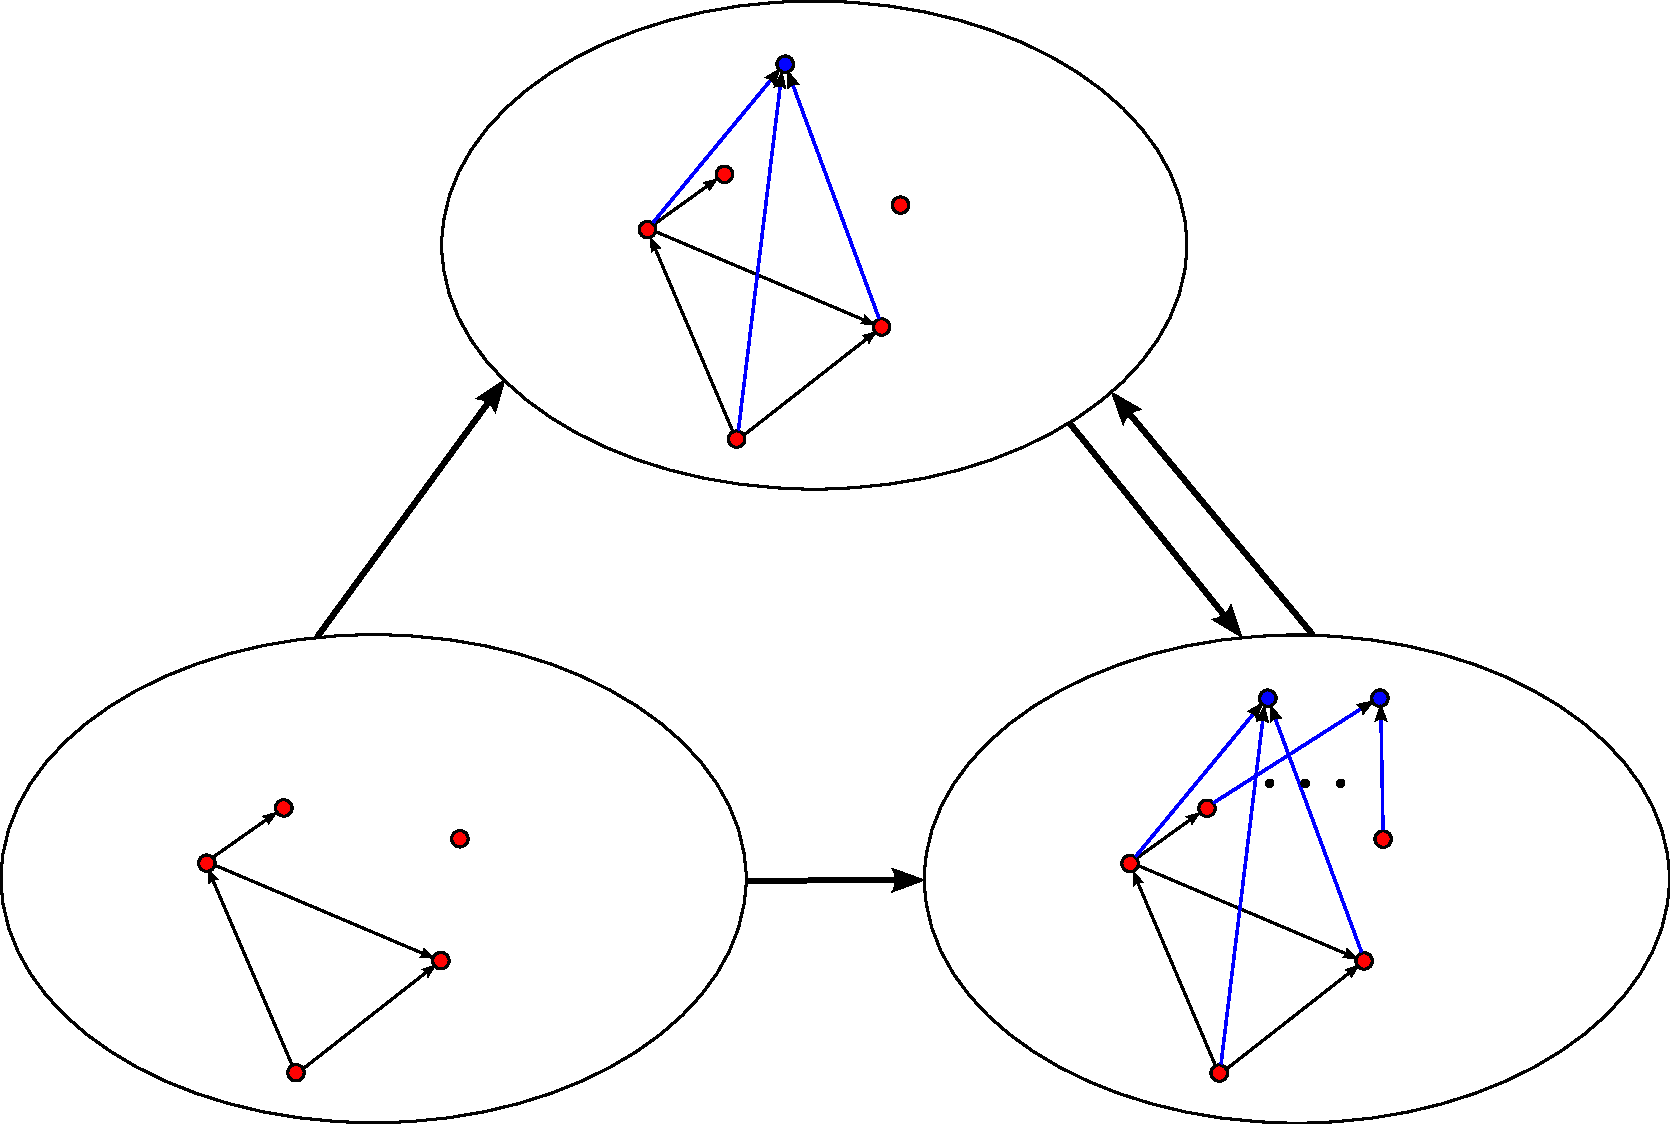
\includegraphics[width=1.0\columnwidth]{fig/graphyonedaext.pdf}
\caption{As a concrete but necessarily incomplete depiction in terms of graphs for intuitive consideration, we can imagine the graph on the left having colimits freely adjoined via Yoneda embedding into the graph on the right (colimits are represented by blue nodes and arrows) and then selecting some of those colimits for inclusion in the category of {\it global} biological information representations. Note that the category of global information representations in this picture is not actually cocomplete as $\mathcal{L}_1$ is assumed to be in figure \ref{fig:ascent}}
\label{fig:graphyonedaext}
\end{figure}

\iftoggle{thmsty}{
\begin{proof}
\label{proof-cocompletion-adjunction}
}{}
A natural transformation can be constructed $\tau : P \rightarrow R(L_1) \in \Mor(Sets^{\mathcal{L}_0^{opp}})$ by defining it on components as set functions parameterized by $L_0 \in \Ob(\mathcal{L}_0)$
$$
\tau_{L_0} : P(L_0) \rightarrow Mor_{\mathcal{L}_1}(A(L_0),L_1)
$$
which is natural in $L_0$ according to the commutativity of the diagram
$$
\xymatrix{
P(L_0) \ar[r]^-{\tau_{L_0}} \ar[d]_{P(u)} & Mor_{\mathcal{L}_1}(A(L_0),L_1) \ar[d]^{A(u)^*} \\
P(L'_0) \ar[r]^-{\tau_{L'_0}} & Mor_{\mathcal{L}_1}(A(L'_0),L_1) }
$$
for all $u:L'_0 \rightarrow L_0 \in \Mor(\mathcal{L}_0)$. $\tau$ is also determined by a family of morphisms in $\Mor(\mathcal{L}_1)$ as
$$
\{ \tau_{L_0}(x):A(L_0) \rightarrow L_1 \}_{(L_0,x)}
$$
indexed by objects $(L_0,x)$ of the category of elements $\int_{\mathcal{L}_0} P$. This construction is natural in objects $(L_0,x)$ in the sense that the diagram
$$
\xymatrix{
A(L_0) \ar@{=}[r] \ar[dd]_{A(u)} & A\pi_P(L_0,x) \ar[rd]^{\tau_{L_0}(x)} \ar[dd]^{u_*} & \\
& & L_1 \\
A(L'_0) \ar@{=}[r] & A\pi_P(L'_0,x') \ar[ru]_{\tau_{L'_0}(x')} &
}
$$
commutes for each morphism $u$.
The functor $L$ is unique for a given $A$ and all functors $A$ from a small category $\mathcal{L}_0$ to a cocomplete category $\mathcal{L}_1$ factor through the Yoneda embedding $PSh$. The Yoneda embedding is thus the universal method of appending colimits to a small category as suggested by the diagram
$$
\xymatrix{
& \mathcal{L}_1 & \\
\mathcal{L}_0 \ar[ru]^{A} \ar[rr]_{PSh} & & \textit{Sets}^{\mathcal{L}_0^{opp}} \ar@{-->}[lu]_{L}
}
$$
which commutes uniquely in $L$ for a given $A$. When $P = Mor(-,L_0) = PSh(L_0)$, the corresponding category of elements $\int_{\mathcal{L}_0} P$ has a terminal object $1_{L_0} : L_0 \rightarrow L_0 \in P(L_0)$. In this case the colimit of $A \circ \pi_P$ is its value on $1_{L_0}$, $L \circ PSh(L_0) \cong A \pi_P (L_0,1_{L_0}) = A(L_0)$ demonstrating the commutativity of the diagram. This construction is referred to as Yoneda extension~\cite{Lane1998,MacLane1992}. Figure \ref{fig:graphyonedaext} presents an intuitive, but imprecise, picture exemplifying some salient features of this construction in terms of directed graphs, which are commonly used to represent {\it network} data pertaining to various molecular, organismal, and ecological aspects of biological systems. 

\iftoggle{thmsty}{
\end{proof}
}

Keeping in mind that $A \cong L \circ PSh$, the functor $R$ can be constructed directly as
\begin{eqnarray*}
R(L_1)(L_0) & \cong & Mor_{\textit{Sets}^{\mathcal{L}_0^{opp}}}(PSh( L_0),R(L_1)),\\
		    & \cong & Mor_{\mathcal{L}_1}(L(PSh(L_0)),L_1),\\
   		    & \cong & Mor_{\mathcal{L}_1}(A(L_0),L_1).
\end{eqnarray*}
So we can simply define $R$ according to
$$
R(L_1)(L_0) = Mor_{\mathcal{L}_1}(A(L_0),L_1),
$$
giving presheaves on $\mathcal{L}_0$ when taken to be parametric in $L_0$.
We can now demonstrate that $L$ and $R$ are indeed adjoint functors %Awodey 9.6 p.200
\begin{eqnarray*}
Nat(P,R(L_1)) & \cong &  Mor_{\textit{Sets}^{\mathcal{L}_0^{opp}}} \left( \lim\limits_{\overrightarrow{j \in \int_{\mathcal{L}_0} P}} PSh (L_{0}^j),R(L_1) \right) ,\\	
			  & \cong &  \lim\limits_{\overleftarrow{j \in \int_{\mathcal{L}_0} P}} Mor_{\textit{Sets}^{\mathcal{L}_0^{opp}}} \left( PSh (L_{0}^j),R(L_1) \right) ,\\
			  & \cong &  \lim\limits_{\overleftarrow{j \in \int_{\mathcal{L}_0} P}} \left( R(L_1)(L_{0}^j) \right) ,\\
  			  & \cong &  \lim\limits_{\overleftarrow{j \in \int_{\mathcal{L}_0} P}} Mor_{\mathcal{L}_1} \left( A (L_{0}^j),L_1 \right) ,\\
  			  & \cong &  Mor_{\mathcal{L}_1} \left( \lim\limits_{\overrightarrow{j \in \int_{\mathcal{L}_0} P}} A (L_{0}^j),L_1 \right) ,\\
  			  & \cong &  Mor_{L_1}(L(P),L_1).
\end{eqnarray*}
There is thus a bijection
$$
Nat_{\textit{Sets}^{\mathcal{L}_0^{opp}}} (P,R(L_1)) \cong Mor_{L_1}(L(P),L_1),
$$
which is natural in both $P$ and $L_1$ demonstrating the adjoint relationship $L \dashv R$.

\begin{figure}
\noindent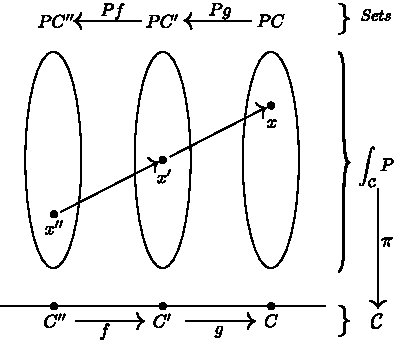
\includegraphics[width=0.8\columnwidth]{fig/catofel.pdf}
\caption{The category of elements of a presheaf functor. Adapted from~\cite{Awodey2006}.}
\label{fig:catofel}
\end{figure}

\section{A topological framework modelling intrinsic integration of biological information}

In order to be able to represent objects and their interactions in the category representing biological entities in terms of global information representations in terms of diagrams modeled in the category of local information representations we make use of a generalized form of topology that can be applied to any category meeting some constraints and that can be specialized to, for example, the case in which objects and morphisms of the category are modelled in terms of a particular type of algebraic structure. This construction develops a method of defining a {\it covering system} composed of interacting entities in the category representing interactions among local information representations that can be used to establish a decomposition of objects in the category representing interactions among global information representations that may each rely on a certain type of composition of local interactions with respect to a particular model of a biological system. We first give a conceptual overview of the standard concepts of {\it sieve}, {\it Grothendieck topology}, {\it site}, and {\it sheaf} for an arbitrary category $\cC$ and then explain how covering sieves on $\mathcal{L}_0$ defined in terms of epimorphic families of morphisms in $\mathcal{L}_1$ provides a Grothendieck topology on $\mathcal{L}_0$, which induces a site and sheaves on $\mathcal{L}_0$. Sheaves on $\mathcal{L}_0$ can be shown to precisely encode the category $\mathcal{L}_1$. The theoretical constraints necessary to ensure the equivalence between information represented in terms of sheaves on the category $\mathcal{L}_0$ and information represented in terms of the category $\mathcal{L}_1$ provide a framework for understanding models of hierarchically organized systems. The process of transforming the category $\mathcal{L}_0$ into its category of sheaves may then provide broad but precise insight into the nature of constraints contextualizing transitions in hierarchical organization that have occurred in the course of biological evolution.

\iftoggle{thmsty}{
\begin{definition}
\label{definition-sieve}
}{}
For any category $\cC$ and $c \in \Ob(\cC)$ a {\it sieve} $S$ on $c$ is a collection in $\Mor(\cC)$ with codomain $c$ such that for $f,g \in \Mor(\cC)$
$$
f \in S \Rightarrow f \circ g \in S
$$
whenever there is a $g \in \Mor(\cC)$ such that $cod(g)=dom(f)$. Any sieve can be restricted to a sieve on the domain of a map whose codomain is the object of the sieve. If $S$ is a sieve on $c$ and $h:d \rightarrow c \in \Mor(\cC)$ with $cod(h)=c$ then
$$
h^* (S) \equiv \{ g \, | \, cod(g)=d, h \circ g \in S \}
$$
is a sieve on $d$.
\iftoggle{thmsty}{
\end{definition}
}

\begin{figure}
\noindent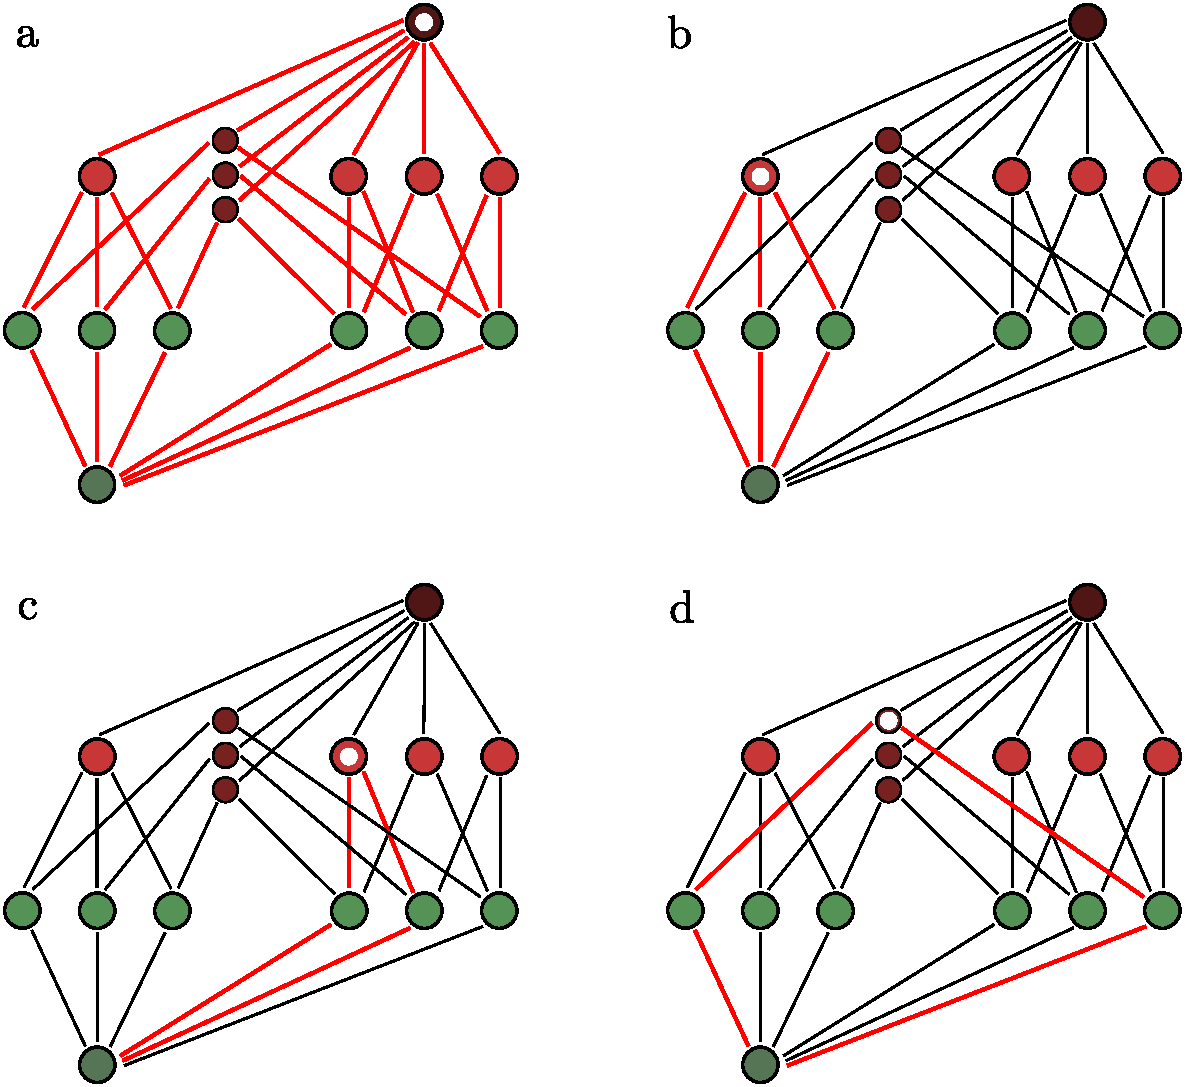
\includegraphics[width=1.0\columnwidth]{fig/sieveHasseNoNum.pdf}
\caption{Sieves conceptualized on {\it Hasse diagrams} of an algebraic lattice. All edges are directed from bottom to top. Red edges are part of a sieve on an object represented by a node in the lattice. Black edges are part of the lattice but not part of the sieve under consideration. (a) shows the maximal sieve on the lattice, which is equivalent to a sieve on the object marked with a white dot. (b), (c), and (d) show maximal sieves on the respective objects marked with white dots.}
\label{fig:sieve}
\end{figure}

A (maximal) sieve is thus a collection of (all) morphisms impinging on a given object upon which it is defined. Examples of sieves on an algebraic lattice are shown in figure \ref{fig:sieve}. There is a simple connection between sieves and the Yoneda embedding $PSh:\cC \rightarrow \textit{Sets}^{\cC^{opp}}$. A sieve on $c$ is a subfunctor $Sc \subseteq hom(-,c)$ of the functor in the presheaf category on $\cC$ that is represented by $c \in \Ob(\cC)$. Placing constraints on such sieves enables the definition of an abstract notion of topology on a category.

\iftoggle{thmsty}{
\begin{definition}
\label{definition-grothendieck-topology}
}{}
A {\it Grothendieck topology} on a category $\cC$ is a function $J$ that assigns a collection $J(c)$ of sieves on $c$ to each $c \in \Ob(\cC)$ such that conditions of maximality, stability and transitivity are satisfied respectively
\begin{enumerate}
\item the maximal sieve $M_c = \{f \, | \, cod(f) = c\} \in J(c)$,
\item for $S \in J(c)$, $f^*(S) \in J(d)$ for any $f:d \rightarrow c \in \Mor(\cC)$,
\item for $S \in J(c)$, $R \in J(c)$ for any sieve $R$ on $c$ with $f^* (R) \in J(d)$ for all $f:d \rightarrow c \in S$.
\end{enumerate}
Sieves $S$ in $J(c)$ for an object $c \in \Ob(\cC)$ are referred to as $J-covering$ sieves.
\iftoggle{thmsty}{
\end{definition}
}

\iftoggle{thmsty}{
\begin{definition}
\label{definition-basis}
}{}
A {\it basis} for a topology on a category $\cC$ that has pullbacks (see Appendix \ref{app:CatTh}) is a function $B$ that assigns to each object $c \in \Ob(\cC)$ a collection of families $\{c_i \rightarrow c \}$ of morphisms referred to as {\it covering families} in $B(c)$ such that
\begin{enumerate}
\item every family consisting of a single isomorphism $\{ d \cong c \}$ is a covering family in $B(c)$
\item if $\{f_i:c_i \rightarrow c \}$ is a covering family and $g:d \rightarrow c$ is any morphism in $\Mor(\cC)$ then $\{g^* c_i \rightarrow d \}$ is a covering family in $B(d)$ of $d$, which means that the collection of covering families is stable under pullbacks
\item if $\{f_i : c_i \rightarrow c \}_{i \in I}$ is a covering family and $\{ g_{i,j} : c_{i,j} \rightarrow c_i \}_{j \in J_i}$ then the family of composites $\{ f_i \circ g_{i,j} : c_{i,j} \rightarrow c_i \rightarrow c \}_{i \in I, j \in J_i}$ is a covering family in $B(c)$
\end{enumerate}
\iftoggle{thmsty}{
\end{definition}
}

\iftoggle{thmsty}{
\begin{definition}
\label{definition-site}
}{}
A pair $(\cC,J)$ or $(\cC,B)$ consisting of a category $\cC$ and a Grothendieck topology $J$ on $\cC$ or a basis $B$ for such a topology is referred to as a {\it site}. If $S \in J(c)$, then $S$ is a {\it covering sieve} of $c$. If $B$ is a basis on $\cC$, then $B$ is said to {\it generate} a topology $J$ according to the equivalence between the statements that a sieve $S$ is a $J$-cover and that a sieve $S$ contains an associated $B$-cover
$$
S \in J(c) \Longleftrightarrow \exists Q \in B(c), \,\,\, Q \subseteq S.
$$
\iftoggle{thmsty}{
\end{definition}
}

\iftoggle{thmsty}{
\begin{definition}
\label{definition-sheaves}
}{}
Given a basis for, $B$, or an explicit Grothendieck topology, $J$, on a category $\cC$ we can define necessary conditions in order for presheaves $P$ in the presheaf category $\textit{Sets}^{\cC^{opp}}$ to be sheaves on the site $(\cC,J)$. If in addition to $P$ we have the sieve $S$ that is a cover of an object $c \in \Ob(\cC)$, then we can define a {\it matching family} for $S$ from elements of $P$ as a function assigning to each $f:d \rightarrow c \in S$ an element $x_f \in P(d)$ such that
$$
\forall g:e \rightarrow d \in \Mor(\cC), \,\,\, x_f \cdot g = x_{fg},
$$
where $x_f \cdot g \equiv P(g)(x_f)$ and $fg \in S$. We can further define an {\it almagamation} of a matching family as a single element $x \in P(c)$ such that
$$
\forall f \in S, \,\,\, x \cdot f = x_f,
$$
implying that $P(f)(x)=x_f$ and thus $P(g)(P(f)(x))=x_{fg}$. $P$ is then a {\it sheaf} for $J$ when every matching family for all covers of all objects in $\Ob(\cC)$ have a unique amalgamation.
\begin{displaymath}
\xymatrix{
e \ar[r]^-{g} & d \ar[r]^-{f} & c\\
P(e) & P(d) \ar[l]_-{P(g)} & P(c) \ar[l]_-{P(f)}\\
x_f \cdot g = x_{fg} & x \cdot f = x_f \ar@{|->}[l]_-{P(g)} & x \ar@{|->}[l]_-{P(f)}
}
\end{displaymath}

A sieve $S$ on an object $c$ is a subfunctor of the functor represented by $c$ under the Yoneda embedding. This is to say that $S \subseteq h_c = hom(-,c)$. In this case, $P$ is a sheaf if and only if for every covering sieve $S$ on $c$ the inclusion $S \hookrightarrow P$ induces an isomorphism $hom(S,P) \cong hom(h_c,P)$. This can also be expressed as the equalizer
\begin{displaymath}
\xymatrix{
P(c) \ar[r]^-{e}
&
\prod\limits_{f \in S}
P(dom \, f)
\ar@<1ex>[r]^-{p} \ar@<-1ex>[r]_-{a}
&
\prod\limits_{\substack{f,g \,\,\, f \in S \\ dom \, f=cod \, g}}
P(dom \, g)
}
\end{displaymath}
\noindent for each $c \in \Ob(\cC)$ and each cover $S \in J(c)$. $e$ refers to $e(x)=\{x \cdot f\}_f = \{P(f)(x)\}_f$, $p$ refers to composition in $\cC$ as $p( \mathbf{x} )_{f,g} = x_{fg}$, and $a$ refers to the action of $\cC$ on $P$ as $a( \mathbf{x} )_{f,g} = x_f \cdot g$ for $\mathbf{x} = \{ x_f \}_{f \in S}$. Given that the equalizer condition, $p \circ e = a \circ e \Leftrightarrow p=a$, is satisfied for a cover $S$ then every family for $S$ has a unique amalgamation and $P$ is thus a sheaf with respect to the cover $S$.

We may express the sheaf condition in terms of a basis $B$ for a topology $J$ generated by $B$ on a category $\cC$, but then we require $\cC$ to have pullbacks. If $Q = \{ f_i : c_i \rightarrow c \}_{i \in I}$ is a B-cover of $c$ a family of elements $x_i \in P(c_i)(i \in I)$ is a matching family for $Q$ if $ x_i \cdot \pi_{ij}^1 = x_j \cdot \pi_{ij}^2$ for all $i,j \in I$. $\pi^1$ and $\pi^2$ are defined as
\begin{displaymath}
\xymatrix{
c_i \times_c c_j \ar[r]^-{\pi_{ij}^2} \ar[d]_{\pi_{ij}^1} & c_j \ar[d]^{f_j} \\
c_i \ar[r]^{f_i} & c
}
\end{displaymath}
which has a corresponding diagram in terms of sets given a presheaf $P$
\begin{displaymath}
\xymatrix{
P(c_i \times_c c_j)  & P(c_j) \ar[l]_-{P(\pi_{ij}^2)}  \\
P(c_i) \ar[u]^-{P(\pi_{ij}^1)}  & P(c) \ar[l]^{f_i} \ar[u]_{f_j}
}
\end{displaymath}
\noindent Now again, a presheaf $P \in \textit{Sets}^{\cC^{opp}}$ is a sheaf for the topology $J$ generated by the basis $B$ if and only if for any cover $\{ f_i : c_i \rightarrow c \}_{i \in I}$ in $B$ any matching family $\{ x_i \}_i$ has a unique amalgamation $x \in P(c)$ such that $x \cdot f_i = x_i$ for all $i \in I$. This condition can also be expressed in terms of an equalizer (see Appendix \ref{app:CatTh})
\begin{displaymath}
\xymatrix{
P(c) \ar[r]
&
\prod\limits_{i \in I}
P(c_i)
\ar@<1ex>[r]^-{p_1} \ar@<-1ex>[r]_-{p_2}
&
\prod\limits_{i,j \in I \times I} P(c_i \times_c c_j)
}
\end{displaymath}
\noindent The morphism $e$ refers to $e(x) = \{ x \cdot f_i \}_i$, $p_1$ refers to $p_1(\{ x_i \})_{i,j} = x_i \cdot \pi_{ij}^1$, and $p_2$ refers to $p_2(\{x_i\})_{i,j} = x_j \cdot \pi_{ij}^{2}$.
\iftoggle{thmsty}{
\end{definition}
}

We now have the necessary machinery in place to explain how covering sieves on $\mathcal{L}_0$ defined in terms of epimorphic families of morphisms in $\mathcal{L}_1$ provides a Grothendieck topology on $\mathcal{L}_0$, thereby inducing a site and sheaves on $\mathcal{L}_0$, which can be shown to precisely encode the category $\mathcal{L}_1$.

\section{Coherence constraints on emerging transitions in hierarchical organization of biological systems}

This section relies on the proof of Giraud's theorem in~\cite{MacLane1992}. Given a functor $A: \mathcal{L}_0 \rightarrow \mathcal{L}_1$, recall the adjunction $L_A \dashv R_A$ between the category of presheaves on the local category $\mathcal{L}_0$ and the global category $\mathcal{L}_1$:
$$
L_A: \textit{Sets}^{\mathcal{L}_0^{opp}} \leftrightarrows \mathcal{L}_1 :R_A.
$$
We can describe the adjoint pair parameterized by a presheaf $P \in \textit{Sets}^{\mathcal{L}_0^{opp}}$, an object $L_1 \in \Ob(\mathcal{L}_1)$ and an object $L_0 \in \Ob(\mathcal{L}_0)$ as
\begin{eqnarray*}
L_A(P) &=& \lim\limits_{\longrightarrow} \left( \int_{\mathcal{L}_0} P \xrightarrow{\pi_P} \mathcal{L}_0 \xrightarrow{A} \mathcal{L}_1 \right),\\
R_A(L_1)(L_0) &=& Mor_{\mathcal{L}_1}(A(L_0),L_1).
\end{eqnarray*}
The functor $L_A$, because colimits can generally be expressed in terms of coequalizers, can also be constructed as a coequalizer for each presheaf $P$
\begin{displaymath}
\xymatrix{
\coprod\limits_{\substack{u : L'_0 \rightarrow L_0 \\ p \in P(L_0)}}
A(L'_0)
\ar@<1ex>[r]^-{\theta} \ar@<-1ex>[r]_-{\tau}
&
\coprod\limits_{\substack{L_0 \\ p \in P(L_0)}}
A(L_0)
\ar[r]
&
P \otimes_{\mathcal{L}_0} A
}
\end{displaymath}
where $P \otimes_{\mathcal{L}_0} A = L_A(P)$.

For a suitable topology $J$ on $\mathcal{L}_0$, the functor $R_A = \Mor_{\mathcal{L}_1}(A(-),-)$ sends $L_1 \in \Ob(\mathcal{L}_1)$ into sheaves (as opposed to mere presheaves) on $\mathcal{L}_0$. $J$ is defined by specifying that a sieve $S(L_0)$ on an object $L_0 \in \mathcal{C}$ is a cover of $L_0$ when the morphisms $g_i : M_0^i \rightarrow L_0 \in S(L_0)$ form an epimorphic family in $\mathcal{L}_1$. The morphisms $g_i$ are components of a morphism defined on the coproduct
$$
b_{S(L_0)} : \coprod\limits_{g_i \in S(L_0)} M_0^i \longrightarrow L_0
$$
over $S(L_0)$. $S(L_0)$ is defined to cover $L_0$ when $b_{S(L_0)}$ is an epimorphism in $\mathcal{L}_1$ via the functor $A:\mathcal{L}_0 \rightarrow \mathcal{L}_1$.

Since this construction is parametric over $L_0 \in \Ob(\mathcal{L}_0)$ and satisfies the maximality, stability and transitivity conditions, this defines a Grothendieck topology on $\mathcal{L}_0$. The conditions of maximality, stability under pullback, and transitivity that ensure the sieve is a Grothendieck topology can all be checked. Roughly, the maximality condition is satisfied by including $1_{L_0} : L_0 \rightarrow L_0$ in the set of morphisms $g_i$ for some $i$. The stability condition requires more detail to verify. Consider the pullback square of an epimorphic family along a morphism $h:L'_0 \rightarrow L_0$
\begin{displaymath}
\xymatrix{
\coprod\limits_{g_i \in S(L_0)} M_0^i \times_{L_0} L'_0 \ar[r]^-{\tilde{g_i}} \ar[d]_{} & L'_0 \ar[d]^{h} \\
\coprod\limits_{g_i \in S(L_0)} M_0^i \ar[r]^-{g_i} & L_0
}
\end{displaymath}
where $\tilde{g_i}$ is also an epimorphism. For $\{ g_i : M_0^i \rightarrow L_0 \}_i \in S(L_0)$ there is an epimorphic family of morphisms $\{ N_0^{ij} \rightarrow M_0^i \times_{L_0} L'_0 \}_{ij}$ with each $N_0^{ij} \in \Ob(\mathcal{L}_0)$. Therefore the composites of these morphisms, $N_0^{ij} \rightarrow M_0^i \times_{L_0} L'_0 \rightarrow L'_0$, for all $i$ and $j$ form an epimorphic family on $L'_0$ contained in the sieve given by the preimage of $h$ on the sieve $S(L_0)$, $h^*(S(L_0))$, and thus $h^*(S(L_0))$ is a cover on $L'_0$, which satisfies the definition of stability of $S(L_0)$ under pullback. Transitivity can also be verified, and thus $J$ is shown to be a Grothendieck topology on $\mathcal{L}_0$ defined in terms of a condition---that sieves on $\mathcal{L}_0$ cover objects in $\mathcal{L}_1$---on its relationship to $\mathcal{L}_1$.

Next we explain the way in which the right adjoint functor parametrically applied to an object $L_1 \in \Ob(\mathcal{L}_1)$, $R_A(L_1) = \Mor_{\mathcal{L}_1}(A(-),L_1): \mathcal{L}_0^{opp} \rightarrow Sets$, is interpreted as a sheaf for the topology $J$ on $\mathcal{L}_0$. Assuming that $\mathcal{L}_1$ is an exact category, the epimorphic family $b_{S(L_0)}$ is the coequalizer of the pullback of $b_{S(L_0)}$ along itself. Since coproducts are stable under pullback for the given assumptions on $\mathcal{L}_1$, 
$$
\left( \coprod\limits_{g'_i \in S(L_0)} M_{0}^{'i} \right) \times_{L_0} \left( \coprod\limits_{g_i \in S(L_0)} M_0^i \right) \cong \coprod\limits_{g'_i , g_i \in S(L_0)} M_0^{'i} \times_{L_0} M_0^i
$$
so that the coequalizer takes the form
\begin{displaymath}
\xymatrix{
\coprod\limits_{g'_i , g_i \in S(L_0)} M_0^{'i} \times_{L_0} M_0^i
\ar@<1ex>[r]^-{\sigma_1} \ar@<-1ex>[r]_-{\sigma_2}
&
\coprod\limits_{g_i \in S(L_0)} M_0^i
\ar[r]^-{b_{S(L_0)}}
&
L_0
}
\end{displaymath}
Due to transitivity of $S(L_0)$ there is an epimorphic family represented by $\{ N_0^{ij} \rightarrow M_0^{'i} \times_{L_0} M_0^i \}_{ij}$ that we can precompose with the coequalizer above yielding
\begin{displaymath}
\xymatrix{
\coprod\limits_{i,j} N_0^{ij}
\ar@<1ex>[r]^-{\alpha} \ar@<-1ex>[r]_-{\beta}
&
\coprod\limits_{g_i \in S(L_0)} M_0^i
\ar[r]^-{b_{S(L_0)}}
&
L_0
}
\end{displaymath}
where there is a commutative diagram in $\mathcal{L}_0$ of the following form
\begin{displaymath}
\xymatrix{
N_0^{ij} \ar[r]^-{h} \ar[d]_{k} & M_0^i \ar[d]^{g_i} \\
M_0^{'i} \ar[r]_-{g'_i} & L_0
}
\end{displaymath}
for each $L_0 \in \Ob(\mathcal{L}_0)$ and where $\alpha$ is associated to $h$ and $\beta$ is associated to $k$.

Now we can apply the functor $R(L_1): \mathcal{L}_0^{opp} \rightarrow Sets$ to the previous coequalizer to obtain
\begin{displaymath}
\xymatrix{
R(L_1)(L_0) \ar[r]
&
\prod\limits_{g_i \in S(L_0)} R(L_1)(M_0^i)
\ar@<1ex>[r]^-{} \ar@<-1ex>[r]_-{}
&
\prod\limits_{i,j} R(L_1)(N_0^{ij})
}
\end{displaymath}
where the arrows are reversed and coproducts exchanged with products producing an equalizer due to the contravariance of the functor $R(L_1)$. This equalizer provides precisely the condition necessary for $R(L_1)$ to satisfy the sheaf condition for the covering sieve $S(L_0)$. Since this construction is parametric in $L_0 \in \Ob(\mathcal{L}_0)$ for a corresponding $L_1 \in \Ob(\mathcal{L}_1)$ of the topology $J$ then $R$ is a $J$-sheaf for the site $(\mathcal{L}_0,J)$. For those cases in which $L_1$ represents an object in $\Ob(\mathcal{L}_0)$ then $R(L_1)$ is equivalent to the functor represented by the object $L_0$ in the presheaf category on $\mathcal{L}_0$. When all representable functors are sheaves, the topology $J$ is referred to as the subcanonical topology on $\mathcal{L}_0$.

Now we consider the unit and counit natural transformations of the adjunction $L_A \dashv R_A$ in the context of the functor $A: \mathcal{L}_0 \rightarrow \mathcal{L}_1$ that enables the transformation of information between the local and the global levels of organization represented by the respective categories. For each $L_1 \in \Ob(\mathcal{L}_1)$, the counit natural transformation
\begin{eqnarray*}
\epsilon_{L_1} &:& L \circ R(L_1) \rightarrow L_1\\
&:& R(L_1) \otimes_{\mathcal{L}_0} A \rightarrow L_1\\
&:& \Mor_{\mathcal{L}_1}(A(-),L_1) \otimes_{\mathcal{L}_0} A \rightarrow L_1
\end{eqnarray*}
can be defined in the coequalizer diagram
\begin{displaymath}
\xymatrix{
\coprod\limits_{\substack{u : L'_0 \rightarrow L_0 \\ r:A(L_0) \rightarrow L_1}}
A(L'_0)
\ar@<1ex>[r]^-{\theta} \ar@<-1ex>[r]_-{\tau}
&
\coprod\limits_{\substack{L_0 \in \Ob(\mathcal{L}_0) \\ r:A(L_0) \rightarrow L_1}}
A(L_0)
\ar[r]^-{\pi} \ar[dr]_-{b_{A(L_0),r}}
&
L_A R_A(L_1) \ar[d]^-{\epsilon_{L_1}}\\
& & L_1
}
\end{displaymath}
where the functor $R_A$ sends objects $L_1 \in \Ob(\mathcal{L}_1)$ to $J$-sheaves on $\mathcal{L}_0$. The morphisms $\theta$ and $\tau$ are respectively associated to the red and blue paths through the diagram
\begin{displaymath}
\xymatrix{
& A(L_0) \ar@[red][d]^{r_i} \\
A(L_0^{'}) \ar@[red][ur]^{A(u)} \ar@[blue][r]_-{r'_i} & L_1
}
\end{displaymath}

The counit $\epsilon_{L_1}$, parametric in $L_1$ is in fact an isomorphism. This can be seen by considering the epimorphic family
$$
b_{A(L_0),r} : \coprod\limits_{\substack{L_0 \in \Ob(\mathcal{L}_0) \\ r:A(L_0) \rightarrow L_1}}
A(L_0) \longrightarrow L_1
$$
in $\mathcal{L}_1$ defined in terms of the functor $A$ and objects $L_0$. This epimorphic family is part of a coequalizer diagram
\begin{displaymath}
\xymatrix{
\coprod\limits_{\substack{i,j}}
A(N_0^{ij})
\ar@<1ex>[r]^-{\alpha} \ar@<-1ex>[r]_-{\beta}
&
\coprod\limits_{\substack{r_i:A(M_0^i) \rightarrow L_1}}
A(M_0^i)
\ar[r]^-{b_{A(M_0^i),r_i}} \ar[dr]_-{\pi}
&
L_1 \ar[d]^-{\epsilon_{L_1}^*}\\
& & L_A R_A(L_1)
}
\end{displaymath}
where $i,j$ indexes commutative diagrams in $\mathcal{L}_1$ of the form
\begin{displaymath}
\xymatrix{
A(N_0^{ij}) \ar@[red][r]^-{h} \ar@[blue][d]_{k} & A(M_0^i) \ar@[red][d]^{r_i} \\
A(M_0^{'i}) \ar@[blue][r]_-{r'_i} & L_1
}
\end{displaymath}
The morphisms $\alpha$ and $\beta$ are respectively associated to the red and blue paths through the diagrams. In this case, $b$ is a coequalizer for $\alpha$ and $\beta$ if and only if it is also a coequalizer for $\theta$ and $\tau$. This fact is evident in the argument \footnote{We allow the substitution rules $L_0 \rightarrow M_0^i$ and $L'_0 \rightarrow M_0^{'i}$ since these differences are merely notational in the sense that they only serve to index objects in the category $\mathcal{L}_0$.} that $(b \theta = b \tau) \Rightarrow (b \alpha = b \beta)$
\begin{eqnarray*}
(b \theta = b \tau) &\Rightarrow & b_{A(M_0^i),r_i} \circ h \\
&=& b_{N_0^{ij},r_i h}\\
&=& b_{N_0^{ij},r'_i k}\\
&=& b_{A(M_0^{'i}),r'_i} \circ k\\
&\Rightarrow & (b \alpha = b \beta)
\end{eqnarray*}
and the converse $(b \alpha = b \beta) \Rightarrow (b \theta = b \tau)$
\begin{eqnarray*}
(b \alpha = b \beta) &\Rightarrow & b_{A(M_0^i),r_i} \circ A(u) \\
&=& b_{A(M_0^{'i}),r_i A(u)}\\
&\Rightarrow & (b \theta = b \tau).
\end{eqnarray*}
This demonstrates that $\epsilon_{L_1}$ is indeed an isomorphism and thus
\begin{eqnarray*}
\epsilon_{L_1} &:& L \circ R(L_1) \cong L_1\\
\epsilon &:& L \circ R \cong 1_{\mathcal{L}_1}
\end{eqnarray*}

We can also demonstrate that the unit of the adjunction is an isomorphism. For any presheaf $Q \in Sets^{\mathcal{L}_0^{opp}}$ the unit of the adjunction $L_A \dashv R_A$ is 

\begin{eqnarray*}
\eta_{Q} &:& Q \rightarrow R \circ L(Q)\\
&:& Q \rightarrow \Mor_{\mathcal{L}_1}(A(-),L_A(Q))\\ 
&:& Q \rightarrow \Mor_{\mathcal{L}_1}(A(-), Q \otimes_{\mathcal{L}_0} A)
\end{eqnarray*}

For the case in which $Q$ is also a sheaf on $\mathcal{L}_0$, it can be dually characterized in terms of a colimit of representable functors $PSh(L_0) = Mor_{\mathcal{L}_0}(-,L_0)$. Additionally, the representable functors are sheaves for the case of the subcanonical topology $J$ on $\mathcal{L}_0$ defined above. Thus if we consider the component of the unit natural transformation at any representable functor we find an isomorphism
$$
\eta_{PSh(L_0)}: PSh(L_0) \cong \Mor_{\mathcal{L}_1}(A(-), PSh(L_0) \otimes_{\mathcal{L}_0} A)
$$
because $PSh(L_0) \cong \Mor_{\mathcal{L}_1}(A(-), A(L_0))$ and $A(L_0) \cong L_A(PSh(L_0))$ in the category $\mathcal{L}_1$. Because the functors $L_A$ and $R_A$ both preserve colimits, any sheaf $Q$ is a colimit of representables, and $\eta_{PSh(L_0)}$ is an isomorphism for representable functors, then $\eta$ is an isomorphism for any sheaf $Q$.

We have demonstrated the counit, $\epsilon$, and the unit $\eta$, to both be isomorphisms for the adjunction $L_A \dashv R_A$ upon restriction from $Sets^{\mathcal{L}_0^{opp}}$ to sheaves on the site defined by $J$ in terms of epimorphic families of morphisms in $\mathcal{L}_1$ for $\mathcal{L}_0$ written as $Sh(\mathcal{L}_0,J)$ 
\begin{eqnarray*}
\eta &:& 1_{Sh(\mathcal{L}_0,J)} \cong R_A \circ L_A,\\
\epsilon &:& L_A \circ R_A \cong 1_{\mathcal{L}_1}.
\end{eqnarray*}
We thus have an equivalence of categories between the category of local representations of biological information and that of global representations (summarized in figure \ref{fig:equivalence})
$$
Sh(\mathcal{L}_0,J) \cong \mathcal{L}_1.
$$
In this light, we can view a process in which interactions among local entities generate higher-level properties that themselves also become entities that may participate in still higher-level processes as requiring the type of coherence precisely specified by the sheaf condition. As biological systems are comprised of structurally nested and functional hierarchies, this constraint, as applied to models of particular biological systems in a category, not limited to but including the graphs which are often produced from network data, may be able to be used to constrain models that are capable of incorporating multiple levels of organization.

\begin{figure}
\noindent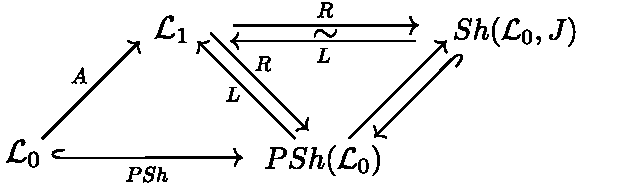
\includegraphics[width=0.9\columnwidth]{fig/equivalence.pdf}
\caption{An extension of the framework for the construction of a mechanism of local-global translation of biological information shown in figure \ref{fig:ascent}.  The functors $R$, and $L$, which were initially defined abstractly have been constructed in terms of $A$ by giving explicit formulas for their action on objects and morphisms. The category of sheaves on the site $(\mathcal{L}_0,J)$, $Sh(\mathcal{L}_0,J)$  has been shown to be equivalent to $\mathcal{L}_1$ via demonstrating that the unit and counit natural transformations of the pair of adjoint functors $R 
\dashv L$ are actually natural isomorphisms.}
\label{fig:equivalence}
\end{figure}
 
\section{Conclusion}

The goal of organizing knowledge about biological systems will ultimately require the development of languages that can be tailored specifically for that task. The purpose of developing such a language is to provide a precise framework for a qualitative phenomenology of biological systems such that, any piece of data that can be collected, can be integrated and used to deduce apparent consequences that in some sense attempt to optimize the production of new or classification of old hypotheses that may be distinguished on that basis. Despite the fact that abstract concepts from pure mathematics have had little explicit coupling to the study of biological systems so far, we find that certain concepts can be adapted to serve as a basis for the development of such a domain-specific language for reasoning about biological systems. In order to realize such a goal, this language will need to be implemented in computational form rather than simply stated in abstract notation; however, clarification of the relationship between purely abstract concepts and concepts abstracted from the study of biological systems can help to make the costly choice of a framework to be implemented for the purposes of knowledge representation.

%------bibliography---%
\bibliographystyle{unsrt}
%\bibliographystyle{natbib} 
\bibliography{bib/books,bib/papers}
%---------------------%


%-----------------------------------------------%
%                   appendix
%-----------------------------------------------%
\appendix

\section{Category theory}\label{app:CatTh}
\iftoggle{thmsty}{
\begin{definition}
\label{definition-category}
}{}
A {\it category} $\mathcal{C}$ is:
\begin{enumerate}
\item A set of objects $\Ob(\mathcal{C})$.
\item For each pair $x, y \in \Ob(\mathcal{C})$ a set of morphisms
$\Mor_\mathcal{C}(x, y)$.
\item For each triple $x, y, z\in \Ob(\mathcal{C})$ a composition
map $ \Mor_\mathcal{C}(y, z) \times \Mor_\mathcal{C}(x, y)
\to \Mor_\mathcal{C}(x, z) $, denoted $(\phi, \psi) \mapsto
\phi \circ \psi$.
\end{enumerate}
Such that these constraints are satisfied:
\begin{enumerate}
\item For every element $x\in \Ob(\mathcal{C})$ there exists a
morphism $\text{id}_x\in \Mor_\mathcal{C}(x, x)$ such that
$\text{id}_x \circ \phi = \phi$ and $\psi \circ \text{id}_x = \psi $.
\item Composition is associative, i.e., $(\phi \circ \psi) \circ \chi =
\phi \circ ( \psi \circ \chi)$.
\end{enumerate}
\iftoggle{thmsty}{
\end{definition}
}

\iftoggle{thmsty}{
\begin{definition}
\label{definition-functor}
}{}
A {\it functor} $F : \mathcal{A} \to \mathcal{B}$
between two categories $\mathcal{A}, \mathcal{B}$ is:
\begin{enumerate}
\item A map $F : \Ob(\mathcal{A}) \to \Ob(\mathcal{B})$.
\item For every $x, y \in \Ob(\mathcal{A})$ a map
$F : \Mor_\mathcal{A}(x, y) \to \Mor_\mathcal{B}(F(x), F(y))$,
denoted $\phi \mapsto F(\phi)$.
\end{enumerate}
These data should be compatible with composition and identity morphisms
in the following manner: $F(\phi \circ \psi) =
F(\phi) \circ F(\psi)$ for a composable pair $(\phi, \psi)$ of
morphisms of $\mathcal{A}$ and $F(\text{id}_x) = \text{id}_{F(x)}$.
\iftoggle{thmsty}{
\end{definition}
}

\iftoggle{thmsty}{
\begin{definition}
\label{definition-transformation-functors}
}{}
Let $F, G : \mathcal{A} \to \mathcal{B}$ be functors.
A {\it natural transformation}, or a {\it morphism of functors}
$t : F \to G$, is a collection $\{t_x\}_{x\in \Ob(\mathcal{A})}$
such that
\begin{enumerate}
\item $t_x : F(x) \to G(x)$ is a morphism in the category $\mathcal{B}$, and
\item for every morphism $\phi : x \to y$ of $\mathcal{A}$ the following
diagram is commutative
$$
\xymatrix{
F(x) \ar[r]^{t_x} \ar[d]_{F(\phi)} & G(x) \ar[d]^{G(\phi)} \\
F(y) \ar[r]^{t_y} & G(y) }
$$
\end{enumerate}
\iftoggle{thmsty}{
\end{definition}
}

\iftoggle{thmsty}{
\begin{definition}
\label{definition-products}
}{}

Let $x, y\in \Ob(\mathcal{C})$,
A {\it product} of $x$ and $y$ is
an object $x \times y \in \Ob(\mathcal{C})$
together with morphisms
$p\in \Mor_{\mathcal C}(x \times y, x)$ and
$q\in\Mor_{\mathcal C}(x \times y, y)$ such
that the following universal property holds: for
any $w\in \Ob(\mathcal{C})$ and morphisms
$\alpha \in \Mor_{\mathcal C}(w, x)$ and
$\beta \in \Mor_\mathcal{C}(w, y)$
there is a unique
$\gamma\in \Mor_{\mathcal C}(w, x \times y)$ making
the diagram
$$
\xymatrix{
w \ar[rrrd]^\beta \ar@{-->}[rrd]_\gamma \ar[rrdd]_\alpha & & \\
& & x \times y \ar[d]_p \ar[r]_q & y \\
& & x &
}
$$
commute.
\iftoggle{thmsty}{
\end{definition}
}

\iftoggle{thmsty}{
\begin{definition}
\label{definition-has-products-of-pairs}
}{}
We say the category $\mathcal{C}$ {\it has products of pairs
of objects} if a product $x \times y$
exists for any $x, y \in \Ob(\mathcal{C})$.
\iftoggle{thmsty}{
\end{definition}
}

\iftoggle{thmsty}{
\begin{definition}
\label{definition-product-category}
}{}
Let $\mathcal{A}$, $\mathcal{B}$ be categories.
The {\it product category} is the category
$\mathcal{A} \times \mathcal{B}$ with
objects
$\Ob(\mathcal{A} \times \mathcal{B}) =
\Ob(\mathcal{A}) \times \Ob(\mathcal{B})$
and
$$
\Mor_{\mathcal{A} \times \mathcal{B}}((x, y), (x', y'))
:=
\Mor_\mathcal{A}(x, x')\times
\Mor_\mathcal{B}(y, y').
$$
Composition of morphisms is defined according to components.
\iftoggle{thmsty}{
\end{definition}
}

\iftoggle{thmsty}{
\begin{definition}
\label{definition-coproducts}
}{}
Let $x, y \in \Ob(\mathcal{C})$,
A {\it coproduct}, or {\it amalgamated sum} of $x$ and $y$ is
an object $x \amalg y \in \Ob(\mathcal{C})$
together with morphisms
$i \in \Mor_{\mathcal C}(x, x \amalg y)$ and
$j \in \Mor_{\mathcal C}(y, x \amalg y)$ such
that the following universal property holds: for
any $w \in \Ob(\mathcal{C})$ and morphisms
$\alpha \in \Mor_{\mathcal C}(x, w)$ and
$\beta \in \Mor_\mathcal{C}(y, w)$
there is a unique
$\gamma \in \Mor_{\mathcal C}(x \amalg y, w)$ making
the diagram
$$
\xymatrix{
& y \ar[d]^j \ar[rrdd]^\beta \\
x \ar[r]^i \ar[rrrd]_\alpha & x \amalg y \ar@{-->}[rrd]^\gamma \\
& & & w
}
$$
commute.
\iftoggle{thmsty}{
\end{definition}
}

\iftoggle{thmsty}{
\begin{definition}
\label{definition-has-coproducts-of-pairs}
}{}
We say the category $\mathcal{C}$ {\it has coproducts of pairs
of objects} if a coproduct $x \amalg y$
exists for any $x, y \in \Ob(\mathcal{C})$.
\iftoggle{thmsty}{
\end{definition}
}

\iftoggle{thmsty}{
\begin{definition}
\label{definition-equalizers}
}{}
Suppose that $X$, $Y$ are objects of a category $\mathcal{C}$
and that $a, b : X \to Y$ are morphisms. We say a morphism
$e : Z \to X$ is an {\it equalizer} for the pair $(a, b)$ if
$a \circ e = b \circ e$ and if $(Z, e)$ satisfies the following
universal property: For every morphism $t : W \to X$
in $\mathcal{C}$ such that $a \circ t = b \circ t$ there exists
a unique morphism $s : W \to Z$ such that $t = e \circ s$.
\iftoggle{thmsty}{
\end{definition}
}
\begin{displaymath}
\xymatrix{
Z \ar[r]^-{e}
&
X \ar@<1ex>[r]^-{a} \ar@<-1ex>[r]_-{b}
&
Y\\
W \ar@{-->}[u]^-{s} \ar[ur]_-{t} & &
}
\end{displaymath}
\iftoggle{thmsty}{
\begin{definition}
\label{definition-coequalizers}
}{}
Suppose that $X$, $Y$ are objects of a category $\mathcal{C}$
and that $a, b : X \to Y$ are morphisms. We say a morphism
$c : Y \to Z$ is a {\it coequalizer} for the pair $(a, b)$ if
$c \circ a = c \circ b$ and if $(Z, c)$ satisfies the following
universal property: For every morphism $t : Y \to W$
in $\mathcal{C}$ such that $t \circ a = t \circ b$ there exists
a unique morphism $s : Z \to W$ such that $t = s \circ c$.
\iftoggle{thmsty}{
\end{definition}
}
\begin{displaymath}
\xymatrix{
X
\ar@<1ex>[r]^-{a} \ar@<-1ex>[r]_-{b}
&
Y \ar[r]^-{c} \ar[dr]_-{t}
&
Z \ar@{-->}[d]^-{s}\\
& & W
}
\end{displaymath}

Examples of equalizers and coequalizers are presented in Figures \ref{fig:equalizer} and \ref{fig:coequalizer} respectively. From these one can recognize intuitive characterizations of each concept. The equalizer $(Z,e)$ is essentially the intersection or solution set of equating two different functions $a=b$. The coequalizer $(Z,c)$ represents the quotient by the smallest equivalence relation that renders $a=b$.

\begin{figure}
\noindent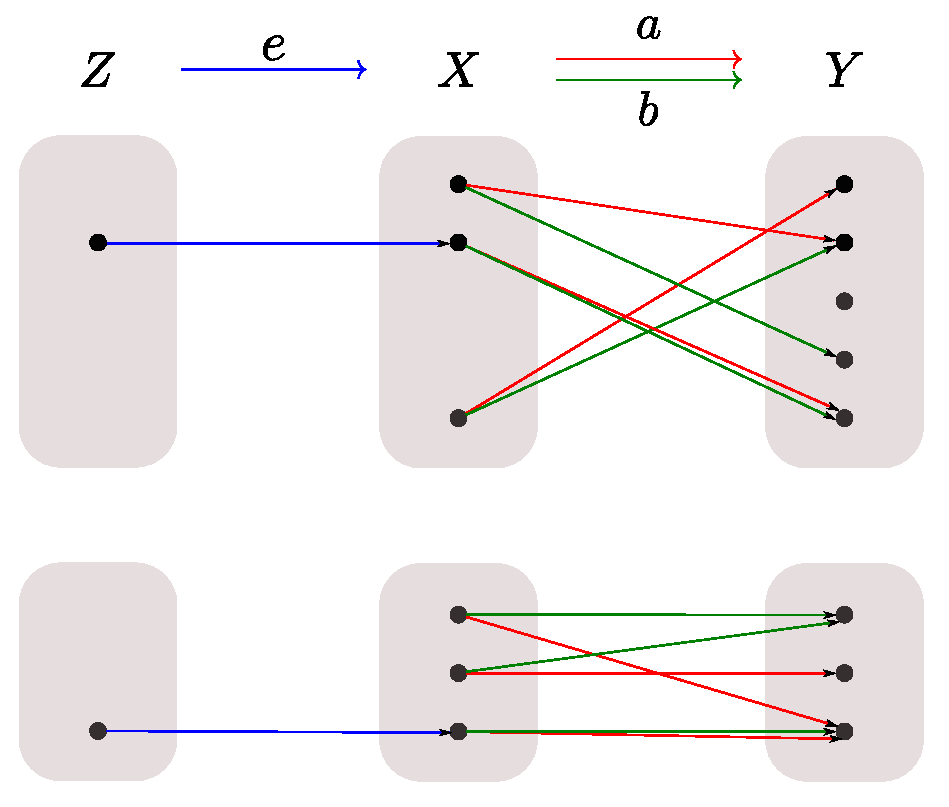
\includegraphics[width=0.9\columnwidth]{fig/equalizer.pdf}
\caption{Examples of equalizers in the category of finite sets.}
\label{fig:equalizer}
\end{figure}

\begin{figure}
\noindent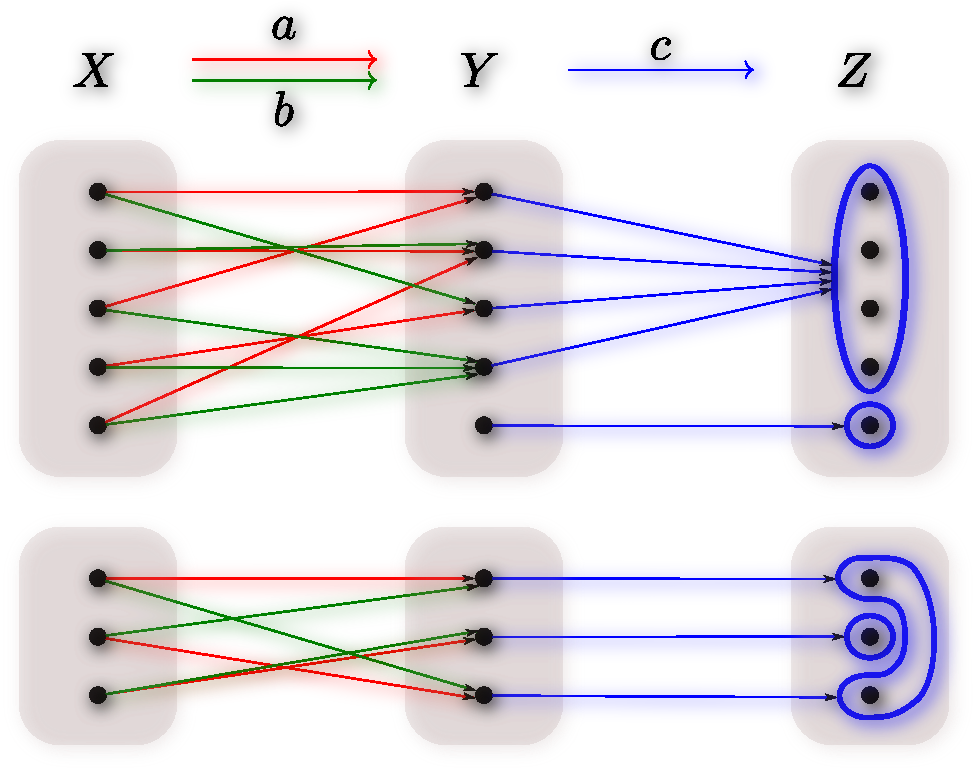
\includegraphics[width=0.9\columnwidth]{fig/coequalizer.pdf}
\caption{Examples of coequalizers in the category of finite sets.}
\label{fig:coequalizer}
\end{figure}

\iftoggle{thmsty}{
\begin{definition}
\label{definition-initial-final}
}{}
Let $\mathcal{C}$ be a category.
\begin{enumerate}
\item An object $x$ of the category $\mathcal{C}$ is called
an {\it initial} object if for every object $y$ of $\mathcal{C}$
there is exactly one morphism $x \to y$.
\item An object $x$ of the category $\mathcal{C}$ is called
a {\it final} object if for every object $y$ of $\mathcal{C}$
there is exactly one morphism $y \to x$.
\end{enumerate}
\iftoggle{thmsty}{
\end{definition}
}

\noindent For example, in \textit{Sets} the empty set $\emptyset$ is the unique
initial object and any {\it singleton} set, a set with one element,
is a final object.

%definitions of pullbacks and pushouts
\iftoggle{thmsty}{
\begin{definition}
\label{definition-fibre-products}
}{}
Let $x, y, z\in \Ob(\mathcal{C})$,
$f\in \Mor_\mathcal{C}(x, y)$
and $g\in \Mor_{\mathcal C}(z, y)$.
A {\it fibre product} of $f$ and $g$ is
an object $x \times_y z\in \Ob(\mathcal{C})$
together with morphisms
$p\in \Mor_{\mathcal C}(x \times_y z, x)$ and
$q\in\Mor_{\mathcal C}(x \times_y z, z)$ making the diagram
$$
\xymatrix{
x \times_y z \ar[r]^{q} \ar[d]_p
&
z \ar[d]^{g}
\\
x \ar[r]^{f}
&
y
}
$$
commute, and such that the following universal property holds: for
any $w\in \Ob(\mathcal{C})$ and morphisms
$\alpha \in \Mor_{\mathcal C}(w, x)$ and
$\beta \in \Mor_\mathcal{C}(w, z)$ with
$f \circ \alpha= g\circ \beta$
there is a unique
$\gamma\in \Mor_{\mathcal C}(w, x \times_z y)$ making
the diagram
$$
\xymatrix{
w \ar[rrrd]^\beta \ar@{-->}[rrd]_\gamma \ar[rrdd]_\alpha
&
&
\\
&
&
x \times_y z \ar[d]_p \ar[r]_q
&
z \ar[d]^{g}
\\
&
&
x \ar[r]^{f}
&
z
}
$$
commute.
\iftoggle{thmsty}{
\end{definition}
}

\noindent
The dual notion to fibre products is that of push outs.

\iftoggle{thmsty}{
\begin{definition}
\label{definition-pushouts}
}{}
Let $x, y, z\in \Ob(\mathcal{C})$,
$f\in \Mor_\mathcal{C}(y, x)$
and $g\in \Mor_{\mathcal C}(y, z)$.
A {\it push out} of $f$ and $g$ is
an object $x\amalg_y z\in \Ob(\mathcal{C})$
together with morphisms
$p\in \Mor_{\mathcal C}(x, x\amalg_y z)$ and
$q\in\Mor_{\mathcal C}(z, x\amalg_y z)$ making the diagram
$$
\xymatrix{
y \ar[r]^{g} \ar[d]_f
&
z \ar[d]^{q}
\\
x \ar[r]^{p}
&
x\amalg_y z
}
$$
commute, and such that the following universal property holds:
For any $w\in \Ob(\mathcal{C})$ and morphisms
$\alpha \in \Mor_{\mathcal C}(x, w)$ and
$\beta \in \Mor_\mathcal{C}(z, w)$ with
$\alpha \circ f = \beta \circ g$ there is a unique
$\gamma\in \Mor_{\mathcal C}(x\amalg_z y, w)$ making
the diagram
$$
\xymatrix{
y \ar[r]^{g} \ar[d]_f
&
z \ar[d]^{q} \ar[rrdd]^\beta
&
&
\\
x \ar[r]^{p} \ar[rrrd]^\alpha
&
x\amalg_y z  \ar@{-->}[rrd]^\gamma
&
&
\\
&&&
w
}
$$
commute.
\iftoggle{thmsty}{
\end{definition}
}

\noindent In the category $\textit{Sets}$ a pullback is a subset of the cartesian product of two sets whereas a pushout is a quotient of the disjoint union of two sets.

%definitions of limits and colimits
Let $\mathcal{C}$ be a category. A {\it diagram} in $\mathcal{C}$ is a functor $M : \mathcal{I} \to \mathcal{C}$. $\mathcal{I}$ is the {\it index category} and $M$ is an $\mathcal{I}$-diagram. $M_i$ denotes the image of the object $i$ of $\mathcal{I}$ in $\cC$. For $\phi : i \to i' \in \Mor(I)$, $M(\phi) : M_i \to M_{i'}$.

\iftoggle{thmsty}{
\begin{definition}
\label{definition-limit}
}{}
A {\it limit} of the $\mathcal{I}$-diagram $M$ in the category
$\mathcal{C}$ is given by an object $\lim_I M$ in $\mathcal{C}$
together with morphisms $p_i : \lim_I M \to M_i$ such that
\begin{enumerate}
\item for $\phi : i \to i'$ a morphism
in $\mathcal{I}$ we have $p_{i'} =  M(\phi) \circ p_i$, and
\item for any object $W$ in $\mathcal{C}$ and any family of
morphisms $q_i : W \to M_i$ such that for all $\phi : i \to i'$
in $\mathcal{I}$ we have $q_{i'} = M(\phi) \circ q_i$ there
exists a unique morphism $q : W \to \lim_I M$ such that
$q_i = p_i \circ q$ for every object $i$ of $\mathcal{I}$.
\end{enumerate}
\iftoggle{thmsty}{
\end{definition}
}

\noindent These conditions are expressed in the commutativity of the diagram
\begin{displaymath}
\xymatrix{
&\ar[ldd]_{q_i} W \ar@{-->}[d]^{q} \ar[rdd]^{q_{i'}} & \\
& \ar[ld]^{p_i} \lim\limits_{\longleftarrow \mathcal{I}} M \ar[rd]_{p_{i'}} &\\
M_i  \ar[rr]_{M(\phi)} & & M_{i'} \\
i \ar[rr]^{\phi} & & i'  
}
\end{displaymath}

\noindent
Limits $(\lim_I M, (p_i)_{i\in \Ob(\mathcal{I})})$ are unique up to unique isomorphism, if they exist at all, according to the uniqueness requirement in the definition. Products of pairs and equalizers are examples of limits. The limit over the empty diagram is a final object of $\cC$. In the category of sets all limits exist. The dual notion is that of colimits.

\iftoggle{thmsty}{
\begin{definition}
\label{definition-colimit}
}{}
A {\it colimit} of the $\mathcal{I}$-diagram $M$ in the category
$\mathcal{C}$ is given by an object $\colim_I M$ in $\mathcal{C}$
together with morphisms $s_i : M_i \to \colim_I M$ such that
\begin{enumerate}
\item for $\phi : i \to i'$ a morphism
in $\mathcal{I}$ we have $s_i = s_{i'} \circ M(\phi)$, and
\item for any object $W$ in $\mathcal{C}$ and any family of
morphisms $t_i : M_i \to W$ such that for all $\phi : i \to i'$
in $\mathcal{I}$ we have $t_i = t_{i'} \circ M(\phi)$ there
exists a unique morphism $t : \colim_I M \to W$ such that
$t_i = t \circ s_i$ for every object $i$ of $\mathcal{I}$.
\end{enumerate}
\iftoggle{thmsty}{
\end{definition}
}

\noindent These conditions are expressed in the commutativity of the diagram
\begin{displaymath}
\xymatrix{
i \ar[rr]^{\phi} & & i' \\
M_i \ar[rd]^{s_i} \ar[rdd]_{t_i} \ar[rr]^{M(\phi)} & & M_{i'} \ar[ldd]^{t_{i'}} \ar[ld]_{s_{i'}}\\
& \lim\limits_{\longrightarrow \mathcal{I}} M \ar@{-->}[d]^{t}& \\
& W &
}
\end{displaymath}
\noindent
Colimits $(\colim_I M, (s_i)_{i\in \Ob(\mathcal{I})})$ are unique up to unique isomorphism by the uniqueness requirement in the definition. Coproducts of pairs and coequalizers are examples of colimits. The colimit over an empty diagram is an initial object of $\mathcal{C}$. All colimits exist in the category of sets.

Combining the diagrams for limit and colimit (in general the objects W refer to different objects in each diagram) demonstrates the reason that limits are often referred to as {\it cones over} a diagram and colimits are referred to as {\it cocones under} a diagram
\begin{displaymath}
\xymatrix{
&\ar[ldd]_{q_i} W \ar@{-->}[d]^{q} \ar[rdd]^{q_{i'}} & \\
& \ar[ld]^{p_i} \lim\limits_{\longleftarrow \mathcal{I}} M \ar[rd]_{p_{i'}} &\\
M_i  \ar[rr]_{M(\phi)} & & M_{i'} \\
i \ar[rr]^{\phi} & & i' \\
M_i \ar[rd]^{s_i} \ar[rdd]_{t_i} \ar[rr]^{M(\phi)} & & M_{i'} \ar[ldd]^{t_{i'}} \ar[ld]_{s_{i'}}\\
& \lim\limits_{\longrightarrow \mathcal{I}} M \ar@{-->}[d]^{t}& \\
& W &
}
\end{displaymath}

We can define a category having functors as objects and natural transformations as morphisms, which is called a functor category, by recognizing that every functor $F$ comes with the {\it identity} transformation $\text{id}_F : F \to F$. In addition, given a morphism of
functors $t : F \to G$ and a morphism of functors $s : E \to F$
then the {\it composition} $t \circ s$ is defined by the rule
$$
(t \circ s)_x = t_x \circ s_x : E(x) \to G(x)
$$
for $x \in \Ob(\mathcal{A})$.
This is a morphism of functors
from $E$ to $G$.
Thus, given categories
$\mathcal{A}$ and $\mathcal{B}$ we obtain the category of functors between $\mathcal{A}$ and
$\mathcal{B}$.

\iftoggle{thmsty}{
\begin{definition}
\label{definition-equivalence-categories}
}{}
An {\it equivalence of categories}
$F : \mathcal{A} \to \mathcal{B}$ is a functor such that there
exists a functor $G : \mathcal{B} \to \mathcal{A}$ such that
the compositions $F \circ G$ and $G \circ F$ are isomorphic to the
identity functors $\text{id}_\mathcal{B}$,
respectively $\text{id}_\mathcal{A}$.
In this case we say that $G$ is a {\it quasi-inverse} to $F$.
\iftoggle{thmsty}{
\end{definition}
}

\iftoggle{thmsty}{
\begin{definition}
\label{definition-adjoint}
}{}
Let $\mathcal{C}$, $\mathcal{D}$ be categories.
Let $F : \mathcal{C} \to \mathcal{D}$ and
$G : \mathcal{D} \to \mathcal{C}$ be functors.
We say that $F$ is a {\it left adjoint} of $G$ or that
$G$ is a {\it right adjoint} to $F$, written $F \dashv G$, if there are bijections
$$
\phi_{c,d}:\Mor_\mathcal{D}(Fc, d)
\simeq
\Mor_\mathcal{C}(c, Gd)
$$
functorial in $c \in \Ob(\mathcal{C})$, and
$d \in \Ob(\mathcal{D})$.
\iftoggle{thmsty}{
\end{definition}
}

Morphisms that are associated with each other according to the bijections of an adjunction are called {\it adjoint transposes} of one another. If $g:Fc \rightarrow d$, $g \in \Mor(\cD)$ then $g^*: c \rightarrow Gd$, $g^* \in \Mor(\cC)$ is given by $\phi_{c,d}(g) = g^*$. Similarly for $f: c \rightarrow Gd$, $f \in \Mor(\cC)$ with $f^*:Fc \rightarrow d$, $f^* \in \Mor(\cD)$ is given by $\phi_{c,d}^{-1}(f) = f^*$. We see then that $g^* = f$ and $f^* = g$.

\iftoggle{thmsty}{
\begin{definition}
\label{definition-opposite}
}{}
Given a category $\mathcal{C}$ the {\it opposite category}
$\mathcal{C}^{opp}$ is the category with the same objects
as $\mathcal{C}$ but all morphisms reversed.
\iftoggle{thmsty}{
\end{definition}
}

\iftoggle{thmsty}{
\begin{definition}
\label{definition-contravariant}
}{}
Let $\mathcal{C}$, $\mathcal{S}$ be categories.
A {\it contravariant} functor $F$
from $\mathcal{C}$ to $\mathcal{S}$
is a functor $\mathcal{C}^{opp}\to \mathcal{S}$.
\iftoggle{thmsty}{
\end{definition}
}

\iftoggle{thmsty}{
\begin{definition}
\label{definition-presheaf}
}{}
Let $\mathcal{C}$ be a category.
\begin{enumerate}
\item A {\it presheaf of sets on $\mathcal{C}$}
or simply a {\it presheaf} is a contravariant functor
$F$ from $\mathcal{C}$ to $\textit{Sets}$. When $F$ is a covariant functor $F : \mathcal{C}^{opp} \rightarrow \textit{Sets}$.
\item The category of presheaves is denoted $\textit{PSh}(\mathcal{C})$.
\end{enumerate}
\iftoggle{thmsty}{
\end{definition}
}

\iftoggle{thmsty}{
\begin{definition}
\label{definition-bifunctor}
}{}
Given categories $\mathcal{C}_1$, $\mathcal{C}_2$, and $\mathcal{D}$. A {\it bifunctor} or binary functor or 2-ary functor or functor of two variables, $F$, is a functor whose domain is the product of two categories $F: \mathcal{C}_1 \times \mathcal{C}_2 \rightarrow \mathcal{D}$.
\iftoggle{thmsty}{
\end{definition}
}

\iftoggle{thmsty}{
\begin{definition}
\label{definition-hom-functor}
}{}
The {\it hom-functor} is a bifunctor defined on the product of a category $\mathcal{C}$ with its self-dual category $\mathcal{C}^{opp}$, which takes values in the category $\textit{Sets}$. Thus for a category $C$ its hom-functor is 
$$
hom(-,-): \mathcal{C}^{opp} \times \mathcal{C} \rightarrow \textit{Sets},
$$
which can be curried in two ways
\begin{eqnarray*}
h^{(-)} &:& \mathcal{C}^{opp} \rightarrow \textit{Sets}^{\mathcal{C}},\\
h_{(-)} &:& \mathcal{C} \rightarrow \textit{Sets}^{\mathcal{C}^{opp}}.
\end{eqnarray*}
The hom-functor maps
\begin{enumerate}
\item objects $(c,c') \in \mathcal{C}^{opp} \times \mathcal{C}$ to the hom-set $\Mor_{\mathcal{C}} (c,c')$, which is the set of morphisms in $\mathcal{C}$ with domain $c$ and codomain $c'$.
\item morphisms 
$$
(f,g):(c,c') \rightarrow (d,d') \in \Mor(\mathcal{C}^{opp} \times \mathcal{C}),
$$
where $f:d \rightarrow c \in \Mor(\mathcal{C})$ and $g:c' \rightarrow d' \in \Mor(\mathcal{C})$, to the set function
\begin{eqnarray*}
\Mor_{\mathcal{C}}(c,c') &\rightarrow& \Mor_{\mathcal{C}}(d,d')\\
(c \rightarrow c') &\mapsto& (d \rightarrow c \rightarrow c' \rightarrow d')
\end{eqnarray*}
\end{enumerate}
\iftoggle{thmsty}{
\end{definition}
}

\iftoggle{thmsty}{
\begin{definition}
\label{definition-representable-functor}
}{}
For a hom-functor $hom(-,-): \mathcal{C}^{opp} \times \mathcal{C} \rightarrow \textit{Sets}$ for $c \in \Ob(\mathcal{C})$ a covariant and contravariant functor can be derived by specializing the hom-functor to morphisms out of or into the object $c$ as
\begin{eqnarray*}
h^c \equiv hom(c,-) &:& \mathcal{C} \rightarrow \textit{Sets},\\
h_c \equiv hom(-,c) &:& \mathcal{C}^{opp} \rightarrow \textit{Sets}.
\end{eqnarray*}
Functors that are isomorphic to $h^c$ or $h_c$ are referred to as {\it corepresentable or representable functors} respectively and $c$ is their {\it representing object}. Note that $h_c \in \Ob(\textit{PSh}(\mathcal{C}))$ and the Yoneda embedding states that $h_c$ extends to a functor $PSh : \mathcal{C} \rightarrow \textit{Sets}^{\mathcal{C}^{opp}}$ that is guaranteed to be full and faithful thereby having $\mathcal{C}$ as a full subcategory of the functor category $\textit{Sets}^{\mathcal{C}^{opp}}$ by the Yoneda lemma.
\iftoggle{thmsty}{
\end{definition}
}

\begin{figure}
\noindent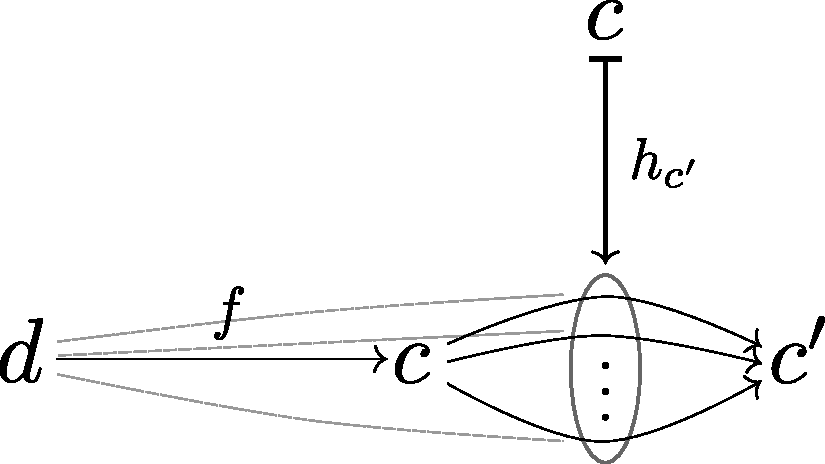
\includegraphics[width=0.7\columnwidth]{fig/hom.pdf}
\caption{The presheaf represented by $c' \in \Ob(\cC)$ is $h_{c'} : \cC^{opp} \rightarrow \textit{Sets}$. It sends objects to the set of morphisms in which they are the domain object with codomain $c'$ and morphisms $f:d \rightarrow c \in \Mor{\cC}$ to set functions $h_{c'} \circ f: \Mor_{\cC}(c,c') \rightarrow \Mor_{\cC}(d,c')$ via pre-composition.}
\label{fig:hom}
\end{figure}

The concrete action of $h_{c'}$ on objects and morphisms in $\cC$ is summarized in Figure \ref{fig:hom}. A complementary characteristic of the Yoneda embedding is that it freely adjoins colimits. As such, one can extract from a presheaf $P \in \textit{Sets}^{\cC^{opp}}$ a diagram in $\cC$ for which $P$ serves as a colimit in $\textit{Sets}^{\cC^{opp}}$. This process follows a simple algorithm:
\begin{enumerate}
\item For all $X \in \Ob(\cC)$ make one copy of $X$ corresponding to each element in $P(X)$.
\item If $f:X \rightarrow Y \in \Mor(\cC)$ consider $P(f):P(Y) \rightarrow P(X)$ and for each $e \in P(Y)$ and $P(f)(e) \in P(X)$ in $\textit{Sets}$ draw the map $f$ from the corresponding $X$ to $Y$ in $\cC$.
\item Follow this procedure for all $f \in \Mor(\cC)$ to reconstruct the diagram in $\cC$ for which $P$ serves as colimit.
\end{enumerate}
The result of this procedure on a simple example from (finite) $\textit{Sets}$ is shown in Figure \ref{fig:presheafeg}.

\begin{figure}
\noindent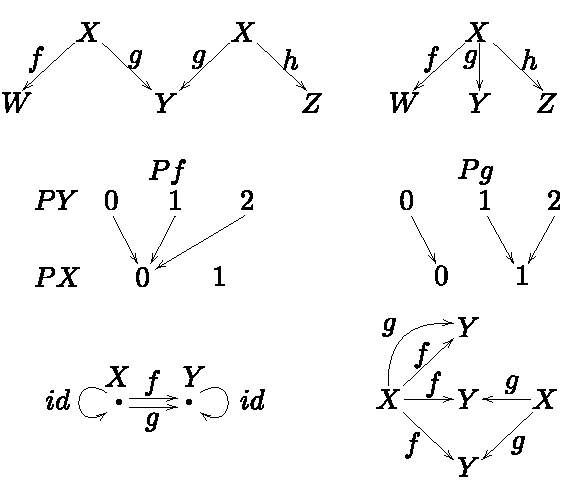
\includegraphics[width=0.9\columnwidth]{fig/presheafeg.pdf}
\caption{The top row shows an example of two diagrams (left and right) that have the same colimit. The middle row provides explicit sets, $PY$ and $PX$, and set maps, $Pf$ and $Pg$, coming from the concrete category represented on the bottom left. The bottom right shows the diagram in $\cC$ reconstructed from $P$ for which $P$ serves as a colimit in $\textit{Sets}^{\cC^{opp}}$.}
\label{fig:presheafeg}
\end{figure}

The preceding definitions are standard category theoretic constructions. Ellerman has proposed an interpretation of adjoint functors, that demonstrates their relevance to the concept of information encoding and decoding (or sending and receiving) in the context of biological systems \cite{Ellerman2005}.

\iftoggle{thmsty}{
\begin{definition}
\label{definition-birepresentable}
}{}
A bifunctor $bif (-,-): \cC^{opp} \times \cD \rightarrow \textit{Sets}$ is said to be {\it birepresentable} if there exists a pair of functors $F:\cC^{opp} \rightleftarrows \cD:G$ where $c \in \Ob(\cC^{opp})$ and $d \in \Ob(\cD)$ gives
\begin{eqnarray*}
b^{c} \equiv bif(c,-) &:& \mathcal{D} \rightarrow \textit{Sets},\\
b_{d} \equiv bif(-,d) &:& \mathcal{C}^{opp} \rightarrow \textit{Sets}.
\end{eqnarray*}
natural in $c$ and $d$ such that $F \dashv G$. The functors $b^{c}$ and $b_{d}$ are defined on
\begin{enumerate}
\item objects for all $c_i \in \Ob(\cC^{opp})$ and for all $d_i \in \Ob(\cD)$
\begin{eqnarray*}
b^{c} (d_i) &=& \Mor_{\cD}(Fc,d_i),\\
b_{d} (c_i) &=& \Mor_{\cC^{opp}}(c_i,Gd).
\end{eqnarray*}
\item morphisms for all $f_{ij}:c_j \rightarrow c_i \in \Mor(\cC^{opp})$ and for all $g_{ij}:d_i \rightarrow d_j \in \Mor(\cD)$ as
\begin{eqnarray*}
b^{c} (g_{ij}) &:& \Mor_{\cD}(Fc,d_i) \rightarrow \Mor_{\cD}(Fc,d_j),\\
b_{d} (f_{ij}) &:& \Mor_{\cC^{opp}}(c_i,Gd) \rightarrow \Mor_{\cC^{opp}}(c_j,Gd).
\end{eqnarray*}
\end{enumerate}
\iftoggle{thmsty}{
\end{definition}
}{}

The composite encoding inspection functor 
$$
b_{(-)} \circ G(-): \cD \rightarrow \cC^{opp} \rightarrow \textit{Sets}
$$
that specifies a set of morphisms in $\cD$ from the perspective of $\cC^{opp}$ is represented by the pair $(F,\eta)$. Likewise, the composite decoding inspection functor 
$$
b^{(-)} \circ F(-): \cC^{opp} \rightarrow \cD \rightarrow \textit{Sets}
$$
that specifies a set of morphisms in $\cC^{opp}$ from the perspective of $\cD$ is represented by the pair $(G,\epsilon)$. Figure \ref{fig:adjunction} summarizes features of the information encoding-decoding adjunction between $F$ and $G$. $F \dashv G$ is thus equivalent to the statement $\phi_{-,-}:b^{(-)} \cong b_{(-)}$.

%\section{Sieves and sheaves}\label{Sheaves}
%\iftoggle{thmsty}{
\begin{definition}
\label{definition-presheaves-injective-surjective}
}{}
Let $\mathcal{C}$ be a category, and let $\varphi : \mathcal{F}
\to \mathcal{G}$ be a map of presheaves of sets.
\begin{enumerate}
\item We say that $\varphi$ is {\it injective} if for every object
$U$ of $\mathcal{C}$ we have $\alpha : \mathcal{F}(U)
\to \mathcal{G}(U)$ is injective.
\item We say that $\varphi$ is {\it surjective} if for every object
$U$ of $\mathcal{C}$ we have $\alpha : \mathcal{F}(U)
\to \mathcal{G}(U)$ is surjective.
\end{enumerate}
\iftoggle{thmsty}{
\end{definition}
}

\iftoggle{thmsty}{
\begin{lemma}
\label{lemma-mono-epi}
}{}
The injective (resp.\ surjective) maps defined above
are exactly the monomorphisms (resp.\ epimorphisms) of
$\textit{PSh}(\mathcal{C})$. A map is an isomorphism
if and only if it is both injective and surjective.
\iftoggle{thmsty}{
\end{lemma}
}{}

\iftoggle{thmsty}{
\begin{definition}
\label{definition-sub-presheaf}
}{}
We say $\mathcal{F}$ is a {\it subpresheaf} of $\mathcal{G}$
if for every object $U \in \Ob(\mathcal{C})$ the set
$\mathcal{F}(U)$ is a subset of $\mathcal{G}(U)$, compatibly
with the restriction mappings.
\iftoggle{thmsty}{
\end{definition}
}

\noindent
In other words, the inclusion
maps $\mathcal{F}(U) \to \mathcal{G}(U)$
glue together to give an (injective) morphism of
presheaves $\mathcal{F} \to \mathcal{G}$.

\iftoggle{thmsty}{
\begin{lemma}
\label{lemma-image}
}{}
Let $\mathcal{C}$ be a category.
Suppose that $\varphi : \mathcal{F} \to \mathcal{G}$ is a
morphism of presheaves of sets on $\mathcal{C}$.
There exists a unique subpresheaf $\mathcal{G}' \subset \mathcal{G}$
such that $\varphi$ factors as
$\mathcal{F} \to \mathcal{G}' \to \mathcal{G}$
and such that the first map is surjective. We
say that $\mathcal{G}'$ is the {\it image of $\varphi$}.
\iftoggle{thmsty}{
\end{lemma}
}

\iftoggle{thmsty}{
\begin{definition}
\label{definition-sieve-s}
}{}
Let $\mathcal{C}$ be a category. Let $U \in \Ob(\mathcal{C})$.
A {\it sieve $S$ on $U$} is a subpresheaf $S \subset h_U$.
\iftoggle{thmsty}{
\end{definition}
}

\noindent
In other words, a sieve on $U$ picks out for each object
$T \in \Ob(\mathcal{C})$ a subset $S(T)$ of the set
of all morphisms $T \to U$. In fact, the only condition
on the collection of subsets
$S(T) \subset h_U(T) = \Mor_\mathcal{C}(T, U)$
is the following rule
\begin{equation}
\label{equation-property-sieve}
\left.
\begin{matrix}
(\alpha : T \to U) \in S(T) \\
g : T' \to T
\end{matrix}
\right\} \Rightarrow
(\alpha \circ g : T' \to U) \in S(T')
\end{equation}

\iftoggle{thmsty}{
\begin{lemma}
\label{lemma-sieves-set}
}{}
Let $\mathcal{C}$ be a category. Let $U \in \Ob(\mathcal{C})$.
\begin{enumerate}
\item The collection of sieves on $U$ is a set.
\item Inclusion defines a partial ordering on this set.
\item Unions and intersections of sieves are sieves.
\item
\label{item-sieve-generated}
Given a family of morphisms $\{U_i \to U\}_{i\in I}$
of $\mathcal{C}$ with target $U$
there exists a unique smallest sieve $S$ on $U$ such that
each $U_i \to U$ belongs to $S(U_i)$.
\item The sieve $S = h_U$ is the maximal sieve.
\item The empty subpresheaf is the minimal sieve.
\end{enumerate}
\iftoggle{thmsty}{
\end{lemma}
}

\iftoggle{thmsty}{
\begin{proof}
}{}
By our definition of subpresheaf, the collection of
all subpresheaves of a presheaf $\mathcal{F}$ is a subset of
$\prod_{U \in \Ob(\mathcal{C})} \mathcal{P}(\mathcal{F}(U))$.
And this is a set. (Here $\mathcal{P}(A)$ denotes
the powerset of $A$.) Hence the collection of sieves on $U$
is a set.

\medskip\noindent
The partial ordering is defined by: $S \leq S'$ if and only if
$S(T) \subset S'(T)$ for all $T \to U$. Notation: $S \subset S'$.

\medskip\noindent
Given a collection of sieves $S_i$, $i \in I$ on $U$ we can
define $\bigcup S_i$ as the sieve with values
$(\bigcup S_i)(T) = \bigcup S_i(T)$ for all
$T \in \Ob(\mathcal{C})$.
We define the intersection $\bigcap S_i$ in the same way.

\medskip\noindent
Given $\{U_i \to U\}_{i\in I}$ as in the statement, consider
the morphisms of presheaves $h_{U_i} \to h_U$. We simply
define $S$ as the union of the images of these maps of presheaves.
\iftoggle{thmsty}{
\end{proof}
}

\iftoggle{thmsty}{
\begin{definition}
\label{definition-sieve-generated}
}{}
Let $\mathcal{C}$ be a category.
Given a family of morphisms $\{f_i : U_i \to U\}_{i\in I}$
of $\mathcal{C}$ with target $U$ we say the sieve
$S$ on $U$ is the {\it sieve  on $U$
generated by the morphisms $f_i$}.
\iftoggle{thmsty}{
\end{definition}
}


\iftoggle{thmsty}{
\begin{definition}
\label{definition-pullback-sieve}
}{}
Let $\mathcal{C}$ be a category.
Let $f : V \to U$ be a morphism of $\mathcal{C}$.
Let $S \subset h_U$ be a sieve. We define the
{\it pullback of $S$ by $f$} to be the sieve
$S \times_U V$ of $V$ defined by the rule
$$
(\alpha : T \to V) \in (S \times_U V)(T)
\Leftrightarrow
(f \circ \alpha : T \to U) \in S(T)
$$
\iftoggle{thmsty}{
\end{definition}
}

$S \times_U V$ can also be referred to as the {\it base change}
of $S$ by $f : V \to U$.

\iftoggle{thmsty}{
\begin{lemma}
\label{lemma-pullback-sieve-section}
}{}
Let $\mathcal{C}$ be a category.
Let $U \in \Ob(\mathcal{C})$.
Let $S$ be a sieve on $U$.
If $f : V \to U$ is in $S$, then
$S \times_U V = h_V$ is maximal.
\iftoggle{thmsty}{
\end{lemma}
}

\iftoggle{thmsty}{
\begin{definition}
\label{definition-topology}
}{}
Let $\mathcal{C}$ be a category.
A {\it topology on $\mathcal{C}$} is given by the following
datum:
\begin{list}{}{}
\item For every $U \in \Ob(\mathcal{C})$
a subset $J(U)$ of the set of all sieves on $U$.
\end{list}
These sets $J(U)$ have to satisfy the following
conditions
\begin{enumerate}
\item For every morphism $f : V \to U$ in $\mathcal{C}$, and
every element $S \in J(U)$ the pullback $S \times_U V$
is an element of $J(V)$.
\item If $S$ and $S'$ are sieves on $U \in \Ob(\mathcal{C})$,
if $S \in J(U)$, and if for all $f \in S(V)$ the pullback
$S' \times_U V$ belongs to $J(V)$, then $S'$ belongs to $J(U)$.
\item For every $U \in \Ob(\mathcal{C})$ the
maximal sieve $S = h_U$ belongs to $J(U)$.
\end{enumerate}
\iftoggle{thmsty}{
\end{definition}
}

\noindent
In this case, the sieves belonging to $J(U)$ are called
the {\it covering sieves}. 

\iftoggle{thmsty}{
\begin{definition}
\label{definition-family-morphisms-fixed-target}
}{}
Let $\mathcal{C}$ be a category.
A {\it family of morphisms with fixed target} in $\mathcal{C}$ is
given by an object $U \in \Ob(\mathcal{C})$, a set $I$ and
for each $i\in I$ a morphism $U_i \to U$ of $\mathcal{C}$ with target $U$.
We use the notation $\{U_i \to U\}_{i\in I}$ to indicate this.
\iftoggle{thmsty}{
\end{definition}
}

\noindent This
notation is meant to suggest an open covering as in topology.

\iftoggle{thmsty}{
\begin{definition}
\label{definition-site-s}
}{}
A {\it site} is given by a category $\mathcal{C}$ and a set
$\text{Cov}(\mathcal{C})$ of families of morphisms with fixed target
$\{U_i \to U\}_{i \in I}$, called {\it coverings of $\mathcal{C}$},
satisfying the following axioms
\begin{enumerate}
\item If $V \to U$ is an isomorphism then $\{V \to U\} \in
\text{Cov}(\mathcal{C})$.
\item If $\{U_i \to U\}_{i\in I} \in \text{Cov}(\mathcal{C})$ and for each
$i$ we have $\{V_{ij} \to U_i\}_{j\in J_i} \in \text{Cov}(\mathcal{C})$, then
$\{V_{ij} \to U\}_{i \in I, j\in J_i} \in \text{Cov}(\mathcal{C})$.
\item If $\{U_i \to U\}_{i\in I}\in \text{Cov}(\mathcal{C})$
and $V \to U$ is a morphism of $\mathcal{C}$ then $U_i \times_U V$
exists for all $i$ and
$\{U_i \times_U V \to V \}_{i\in I} \in \text{Cov}(\mathcal{C})$.
\end{enumerate}
\iftoggle{thmsty}{
\end{definition}
}

We can now define what a sheaf is in two different ways.

\iftoggle{thmsty}{
\begin{definition}
\label{definition-sheaf-sets}
}{}
Let $\mathcal{C}$ be a site, and let $\mathcal{F}$ be a presheaf of sets
on $\mathcal{C}$. We say $\mathcal{F}$ is a {\it sheaf} if
for every covering $\{U_i \to U\}_{i \in I} \in \text{Cov}(\mathcal{C})$
the diagram
\begin{equation}
\label{equation-sheaf-condition}
\xymatrix{
\mathcal{F}(U) \ar[r]
&
\prod\nolimits_{i\in I}
\mathcal{F}(U_i)
\ar@<1ex>[r]^-{\text{pr}_0^*} \ar@<-1ex>[r]_-{\text{pr}_1^*}
&
\prod\nolimits_{(i_0, i_1) \in I \times I}
\mathcal{F}(U_{i_0} \times_U U_{i_1})
}
\end{equation}
represents the first arrow as the equalizer of $\text{pr}_0^*$
and $\text{pr}_1^*$.
\iftoggle{thmsty}{
\end{definition}
}

\iftoggle{thmsty}{
\begin{definition}
\label{definition-sheaf-sets-topology}
}{}
Let $\mathcal{C}$ be a category endowed with a
topology $J$. Let $\mathcal{F}$ be a presheaf of sets
on $\mathcal{C}$.
We say that $\mathcal{F}$ is a
{\it sheaf} on $\mathcal{C}$
if for every $U \in \Ob(\mathcal{C})$ and for
every covering sieve $S$ of $U$ the canonical map
$$
\Mor_{\textit{PSh}(\mathcal{C})}(h_U, \mathcal{F})
\longrightarrow
\Mor_{\textit{PSh}(\mathcal{C})}(S, \mathcal{F})
$$
is bijective.
\iftoggle{thmsty}{
\end{definition}
}

\noindent
The left hand side of the formula equals $\mathcal{F}(U)$ according to the Yoneda lemma. In other words, $\mathcal{F}$ is a sheaf if and only if a section of $\mathcal{F}$
over $U$ is the same thing as a compatible collection of sections
$s_{T, \alpha} \in \mathcal{F}(T)$ parametrized by $(\alpha : T \to U) \in S(T)$, and this for every covering sieve $S$ on $U$.


\end{document}
